% Preamble
\documentclass[a4paper, twoside, 12pt]{report}

% % -------------------- New packages  ----------------------------
% \usepackage{multirow}
%\usepackage{changepage}
%\usepackage{titlesec}
\usepackage{amsmath}
\usepackage{float}
\usepackage{fancyhdr}

\usepackage[linesnumbered,ruled,vlined]{algorithm2e}
\usepackage[noend]{algpseudocode}
\algnewcommand\algorithmicforeach{\textbf{for each}}
\algdef{S}[FOR]{ForEach}[1]{\algorithmicforeach\ #1\ \algorithmicdo}

\usepackage{array}
\newcolumntype{P}[1]{>{\centering\arraybackslash}p{#1}}

\setcounter{secnumdepth}{3}

\usepackage{textcomp}
\usepackage{gensymb}


% % ------------------------------------------------

% Includes
		% UTF-8 encoding, so that yogoou can use characters like ç and ã

\usepackage[T1]{fontenc}				% Same, but for output encoding
\usepackage[utf8]{inputenc}		
\usepackage{tikz}
\def\checkmark{\tikz\fill[scale=0.4](0,.35) -- (.25,0) -- (1,.7) -- (.25,.15) -- cycle;} 
\def\diameter{\tikz\filldraw[fill=white!60,line width=0.15mm](0,0) circle[radius=0.15cm] -- (-0.18,-0.18) -- (-0.19,-0.19) -- (-0.19,-0.19)-- (0.18,0.18) -- cycle;} 

\usepackage[portuges]{babel}	% Still related to the above
\usepackage{acronym}					% List of acronyms
\usepackage{textcomp} 					% Extra characters
\usepackage{graphicx} 					% \includegraphics{}, the most common command to include images in figures
\usepackage{titlesec}					% To manually format the chapter titles
\usepackage[left=3cm,right=2.5cm,top=2.5cm,bottom=2.5cm]{geometry} % Margins, as dictated by the rules
%\usepackage[nottoc,numbib]{tocbibind} 	% Hyperlinks in table of contents, useful for navigation
\usepackage[section]{placeins}			% \FloatBarrier, a useful command when your figures are trying to run away
\usepackage{caption}					% For captioning figures
\usepackage{subcaption}					% Subfigures (the subfigure package is deprecated and should not be used)
\usepackage[toc,page]{appendix}			% Appendices
\usepackage{pdfpages}					% Useful when your appendix is a pre-compiled PDF, such as a whole paper
\usepackage{url}						% Useful when one wants to include URLs in the text
\usepackage[
      colorlinks=true,    			%no frame around URL
      urlcolor=black,    			%no colors
      menucolor=black,    			%no colors
      linkcolor=black,    			%no colors
      citecolor=black,    			%no colors
      bookmarks=true,    			%tree-like TOC
      bookmarksopen=true,    		%expanded when starting
      bookmarksnumbered=true, 		%Put section numbers in bookmarks
      hyperfootnotes=true,    		%no referencing of footnotes, does not compile
      pdfpagemode=UseOutlines,    	%show the bookmarks when starting the pdf viewer
      plainpages=false, 			%solve problem ``destination with the same identifier'' warning
      pdfpagelabels				 	%solve problem ``destination with the same identifier'' warning
]{hyperref} 							% So that our citations look good and still work as links
\usepackage{epigraph}					% For your inspirational quote
\usepackage{etoolbox}
\usepackage{enumitem}
\usepackage{listings,xcolor}
\usepackage{algpseudocode, algorithm2e}
\usepackage{algcompatible}
\usepackage{booktabs}
\usepackage{multirow}
\usepackage{emptypage}
%\usepackage{subfigure}
%\usepackage{fontspec}

\setlength{\parindent}{2em}

\setlength{\headheight}{16pt}
\renewcommand{\baselinestretch}{1.3}	% 1.5 line spacing, as mandated by the rules
%\titleformat{\chapter}[hang] 			% Smaller chapter titles
%{\normalfont\huge\bfseries}{\thechapter}{1em}{}

% Your info goes here
\newcommand{\thesistitle}{Relatório de Estágio MEI-IdC}			% Your work's title
\newcommand{\myname}{João Paulo Lopes Agostinho}				% Your name
\newcommand{\statedate}{Tomar, Março 2020}					% The date, usually "Place, Month Year"
\newcommand{\supervisorname}{Renato Eduardo da Silva Panda, Instituto Politécnico de Tomar}		% Your supervisor's name
%\newcommand{\cosupervisorname}{Professora Doutora Marie Curie}	% Your co-supervisor's name, if any.


\renewcommand\lstlistingname{}
\renewcommand\lstlistlistingname{Algorithms} %!!!!!!!!!!!!!!!!!!!!!!!!!!!!!!!!!!!!!!!!!!!!!!!!!!!!!!!!!!!!!!!!!!!!!!!!!!!!!!!!!!

%\DeclareUnicodeCharacter{00A0}{~}

\makeatletter
\renewcommand*{\cleardoublepage}{\clearpage\if@twoside \ifodd\c@page\else
\hbox{}%
\thispagestyle{empty}%
\newpage%
\if@twocolumn\hbox{}\newpage\fi\fi\fi}
\makeatother

\pagestyle{plain}
\addto\captionsportuges{
  \renewcommand{\contentsname}%
    {ÍNDICE}%
}
\addto\captionsportuges{
  \renewcommand{\listtablename}%
    {ÍNDICE DE TABELAS}%
}
\addto\captionsportuges{
  \renewcommand{\listfigurename}{ÍNDICE DE FIGURAS}
}

\renewcommand\appendixtocname{Apêndice}
\renewcommand\appendixpagename{Apêndice}


% MAIN DOCUMENT
\begin{document}
\pagestyle{headings}
\pagenumbering{roman}

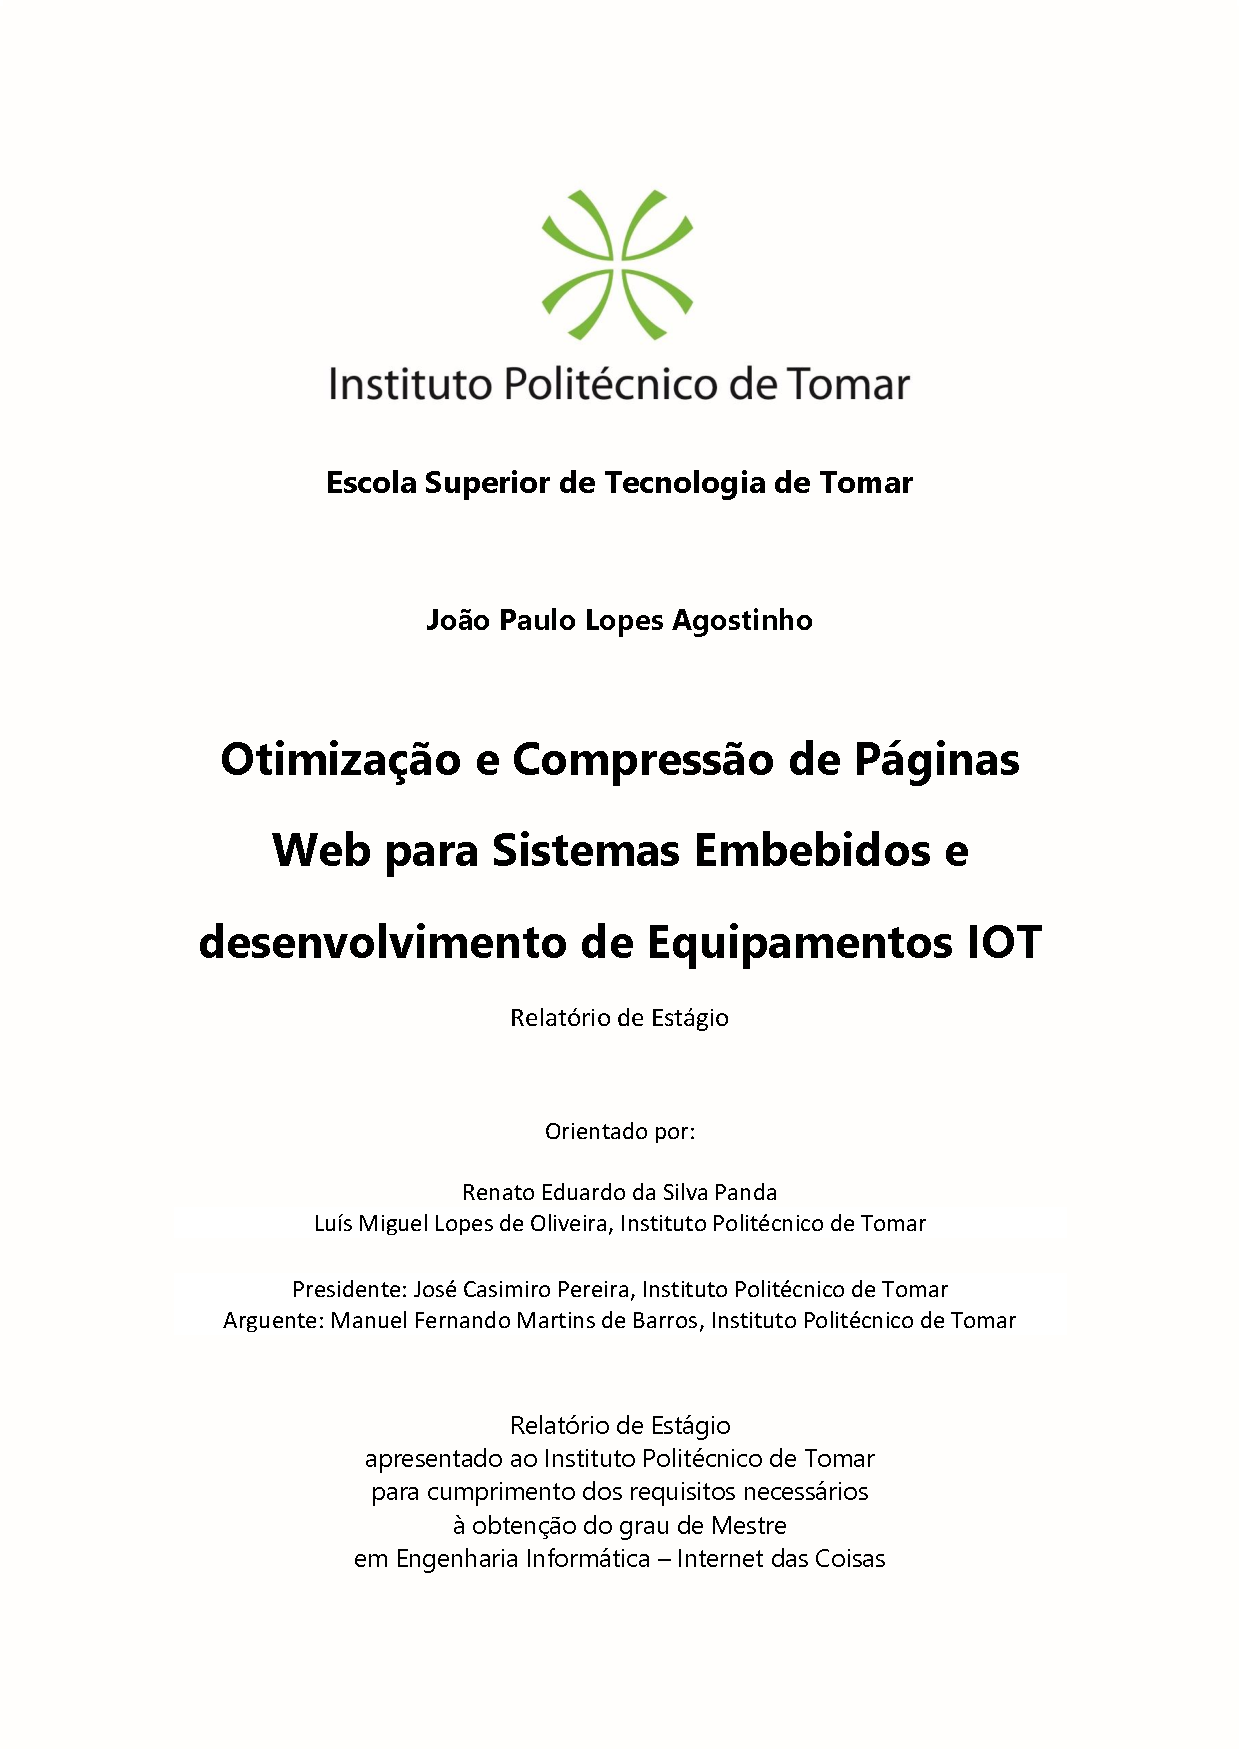
\includepdf[pages={-}]{images/cover/capa.pdf}
% Blank page
\newpage
\thispagestyle{empty}
\mbox{}
% Title page 1
%\begin{titlepage}
\thispagestyle{empty}

\begin{center}
% IPT Logo and Name

\includegraphics[width=0.8\textwidth]{images/logo_ipt.jpg}
% Thesis name
\vspace{1cm}
{\huge{\textbf{\thesistitle}}\par}
\vspace{1.5cm}
{{\large{Dissertação de Mestrado}}\par}

\vspace{1.5cm}
{\large{\textbf{Orientado por:}\\
Prof. Dr. Einstein \\
Prof. Dr. Marie Curie \\
Prof. Dr. Darth Vader
}}

\vspace{1cm}
{\large{\textbf{Juri:} \\
Prof. Dr. Steve Jobs \\
Prof. Dr. Bill Gates \\
Prof. Dr. Mark Zuckerberg
}}

% Final Stuff
\vfill
Dissertação apresentada ao Instituto Politécnico de Tomar para cumprimento dos requisitos necessários à obtenção do grau de Mestre em Engenharia Informática – Internet das Coisas

\vspace{0.5cm}
{\large \statedate\par}


\end{center}
\end{titlepage}  
% Blank page
%\newpage
%\thispagestyle{empty}
%\mbox{}

% Agradecimentos
\titleformat{\chapter}[display]{\rmfamily\Large\bfseries}{\thechapter}{0.5ex}{\centering}[\vspace{-0.5ex}\rule{\textwidth}{0.3pt}]
\chapter*{AGRADECIMENTOS}
\addcontentsline{toc}{chapter}{Agradecimentos}
\titleformat
{\chapter} % command
[display] % shape
{\bfseries\Large\itshape} % format
{Story No. \ \thechapter} % label
{0.5ex} % sep
{
    \rule{\textwidth}{1pt}
    \vspace{1ex}
    \centering
} % before-code
\par\par
Quero agradecer à minha família e amigos, pelo apoio dado nos bons e maus momentos não só durante a vida académica, mas durante toda a minha vida.\par
Aos meus colegas de curso e professores pelos bons tempos que foram passados nas aulas deste Mestrado.\par
Quero agradecer igualmente ao meu orientador, o professor Renato Panda por ser meu orientador e estar sempre disponível para ajudar nesta última fase do Mestrado.\par
À empresa Captemp pela possibilidade de realizar o estágio para conclusão de mais uma etapa da minha vida.\par

% You can add blank pages here, if you like
\newpage\null\thispagestyle{empty}\newpage

% RESUMO
\titleformat{\chapter}[display]{\rmfamily\Large\bfseries}{\thechapter}{0.5ex}{\centering}[\vspace{-0.5ex}\rule{\textwidth}{0.3pt}]
\chapter*{RESUMO}
\addcontentsline{toc}{chapter}{Resumo}
% Resumo em Português

\vspace{1cm}
\noindent
\par Este relatório de estágio foi realizado no âmbito do estágio inserido no Mestrado em Engenharia Informática-Internet das Coisas da Escola Superior de Tecnologia de Tomar do Instituto Politécnico de Tomar, e tem como objetivo colocar em ambiente real os conhecimentos adquiridos no percurso académico.

\par O estágio tem inerente 4 projetos associados à área do IOT e da monitorização de ambientes e/ou objetos com recurso a diversas soluções. O primeiro projeto, referente ao equipamento "Nidus" já existente. Este equipamento disponibilizado em vários modelos permite a ligação de vários tipos de sensores e atuadores  e centralizar o sistema de monitorização. Este equipamento é capaz igualemente a comunicação dos dados para um portal \textit{Cloud} onde é posível analizar os dados enviados pelos vários equipamentos. Neste projeto é necessário a análise do estado atual do projeto e dar continuidade ao suporte do \textit{Front-end} WEB do equipamento. Este projeto pretende estudar e alterar os métodos de desenvolvimento da página referentes á compressão dos ficheiros para reduzir o espaço ocupado pelas páginas WEB em equipamentos de baixos recursos computacionais e armazenamento, a adoção de um melhor método para utilização de imagens nas interfaces WEB em equipamentos com armazenamento limitado e o desenvolvimento de novas funcionalidades tais como um sistema de internacionalização de modo a disponibilizar o equipamento noutros idiomas, sempre tendo em, conta o baixo armazenamneto disponível. Os restantes projetos serão desenvolvidos de raiz durante o estágio  a pedido dos clientes, por soluções à medida, ou quer pela inovação e evolução dos produtos da empresa, e consistem em novos equipamentos para monitorização.

\par O segundo projeto é referente ao desenvolvimento de um equipamento IOT que tire partido das vantagens da nova tecnologia de comunicação o \textit{Narrowband} (NB-IOT). Neste equipamento irá ser possivel adicionar vários sensores já comercializados pela Captemp. O equipamento é capaz de realizar as leituras de todos os sensores connectados, realizar o armazenamento em Log para posterior envio para o portal \textit{Cloud} para consulta futura ou gestão da alarmística correspondente. Este equipamento é igualmente capaz de realizar uma configuração bi-direcional de modo a ser possível realizar a sua configuração através do portal \textit{Cloud}.

\par Paralelamente aos projetos anteriores e com o emergir de novas técnologias tais como os \textit{Beacons Bluetooth Low Energy} e pela sugestão de diversos clientes de uma nova solução de monitorização portátil e simples, foi criado o projeto "Kea Tracker" composto por \textit{Beacons} e uma aplicação \textit{Mobile} para \textit{Smartphones}, responsável por perioódicamente realizar a leitura dos sensores presentes nos \textit{Beacons}, o seu armazenamento e posterior envio para o portal \textit{Cloud}, à semelhança do projeto anterior. Neste projeto o \textit{Beacon} é igualmente capaz de registar em Log interno para caso exista falha de comunicação com a aplicação \textit{Mobile}, posteriormente esses dados serem descarregados quando o \textit{Smartphone} estiver disponível.

\par O último projeto referente deste estágio, foi solicitado pelo cliente que pretende uma plataforma WEB para localizar pessoas em ambientes \textit{indoor}. Esta solução baseia-se no desenvolvimento de uma solução composta por localizadores, \textit{Gateways} e uma plataforma WEB onde seja possível realizar o \textit{Tracking} de pessoas e de objetos em ambientes \textit{indoor} num mapa e assim gerir os tempos de acesso a zonas definidas, criar alertas, ou simplesmente gerir o stock dos armazéns. Este projeto, à semelhança do projeto "Kea Tracker", usa como tecnologia de suporte \textit{Beacons Bluetooth Low Energy} (BLE) para fazer o tracking em tempo real.




\bigskip

\textbf{Palavras chave:}
IOT, Monitorização, Compressão WEB,Compressão de Imagens,NB-IOT,Beacon,BLE, Indoor Tracking, Bluetooth Tracking
\newpage\null\thispagestyle{empty}\newpage 

%ABSTRACT
\titleformat{\chapter}[display]{\rmfamily\Large\bfseries}{\thechapter}{0.5ex}{\centering}[\vspace{-0.5ex}\rule{\textwidth}{0.3pt}]
\chapter*{ABSTRACT}
\addcontentsline{toc}{chapter}{Abstract}
% Abstract in English

\vspace{1cm}
\noindent
\textbf{} 

\par This traineeship report was made in the scope of the traineeship inserted in the master's degree in Computer Engineering -Internet of Things at the School of Technology of Tomar from the Polytechnic Institute of Tomar, and has a goal place in real environment the knowledge acquired in the academic path.

\par The traineeship has inherent 4 associated projects at the area of IOT and the monitoring of environments and/or objects using different solutions. One of the projects, "Nidus" already existed and it is necessary to analyze the project to continue the support of Front-end. In this project, it is necessary to study and change the page development methods related to file compression to reduce the space occupied by the WEB pages, the adoption of a better method for using images on the WEB interfaces on equipment with low resources and the development of new features such as an internalization system in order to make the equipment available in other languages. The remaining projects will be developed from scratch during the traineeship, or by clients requesting custom solutions or by the innovation/evolution of the company's products, and consist of new equipments for monitoring, namely environmental monitoring and Tracking of objects.

\par The second project is relative of the development of an IOT device that takes advantage of the new communication technology NB-IOT. In this equipment it is possible to add several sensors, and the equipment is able to perform the readings of the various sensors, storage in Log for later upload to a Cloud portal for future preview or make alerts.
\par In parallel with the previous project and with the emergence of new technologies such as Bluetooth Low Energy Beacons and the request by several customers for a new portable and simple monitoring solution, the "Kea Tracker" project was created, composed with several Beacons and an application Mobile responsible for reading the sensors present in Beacons and upload them to the Cloud portal. In this project, Beacon must also have an internal Log system for communication failure with the Mobile application.
\par The last project of the traineeship, requested by the client, is based on the development of a solution composed of Sensors and Gateways and a WEB platform that makes it possible to Tracking people and objects in indoor environments and thus manage access times, create alerts, or simply manage the stock of warehouses. This project uses as support technology Bluetooth Low Energy Beacons (BLE) to do real-time tracking.

\bigskip

\textbf{Key words:} 
IOT, Monitoring, WEB Compression, Image Compression, NB-IOT, Beacon, BLE, Indoor Tracking, Bluetooth Tracking
% And here as well
\newpage\null\thispagestyle{empty}\newpage

% INSPIRATIONAL QUOTE
% Setup
\setlength\epigraphwidth{12cm}
\setlength\epigraphrule{0pt}
\makeatletter
\patchcmd{\epigraph}{\@epitext{#1}}{\itshape\@epitext{#1}}{}{}
\makeatother
% Actual Quote
\vspace*{\fill}
\epigraph{"Persistence is the shortest path to success"}{}
{ ---  \textup{Charles Chaplin}}
\vspace*{\fill}
\newpage\null\thispagestyle{empty}\newpage

% TABLE OF CONTENTS

\titleformat{\chapter}[display]{\rmfamily\Large\bfseries}{\thechapter}{0.5ex}{\centering}[\vspace{-0.5ex}\rule{\textwidth}{0.3pt}]
\tableofcontents
\clearpage
% LIST OF ACRONYMS
\chapter*{ACRÓNIMOS}
\addcontentsline{toc}{chapter}{Acrónimos}

\begin{acronym}[list\_acronyms]

%\newacronym{BLE}{BLE}{Bluetooth Low Energy}
%\newacronym{GSM}{GSM}{Global System for Mobile Communications}
%\newacronym{JPG}{JPG}{Joint Photographic Group}
%\newacronym{HTML}{HTML}{HyperText Markup Language
%\newacronym{NB-IOT}{NB-IOT}{Narrowband IoT}
%\newacronym{PNG}{PNG}{Portable Network Graphics}
%\newacronym{RTC}{RTC}{Real Time Clock}
%\newacronym{SVG}{SVG}{Scalable Vector Graphics}


%\printglossary[type=\acronymtype]
\end{acronym}

\addcontentsline{toc}{chapter}{Índice de Figuras}
\listoffigures
\clearpage %\cleardoublepage %for openright
\addcontentsline{toc}{chapter}{Índice de Tabelas}
\listoftables
\clearpage %\cleardoublepage %for openright
% BODY
\newpage
\thispagestyle{empty}
\mbox{}

\fancyhead[LE,RE]{\slshape\rightmark}
\fancyhead[LO,RO]{\slshape\leftmark}
\fancyhead[RE,LO]{}
\pagestyle{fancy}
\titleformat{\chapter}[display]
    {\normalfont\huge\bfseries}{\chaptertitlename\ \thechapter}{20pt}{\Huge}
\titlespacing*{\chapter}{0pt}{0pt}{20pt}

\chapter{Introdução}
\pagenumbering{arabic}
\section{Contextualização}
\par
Atualmente a sociedade vive rodeada de tecnologias indispensáveis e de ambientes que se intitulam inteligentes (\textit{smart}), mas nem sempre foi assim.\par
Desde cedo, mesmo antes de existir tecnologia, o homem tendeu a procurar e encontrar coisas que melhorassem a sua vida e bem-estar pessoal e da sociedade, mas para chegar a humanidade está hoje é necessário recuar na história algum tempo para marcos importantes da tecnologia.\par
Um dos marcos muito importantes para o desenvolvimento dos sistemas embebidos e de sistemas de monotorização foi a invenção dos processadores. Com o surgimento dos processadores começaram a surgir os primeiros sistemas embebidos e sistemas de monotorização. Com o passar dos anos até aos dias de hoje a tecnologia tem vindo a evoluir e por consequência os sistemas também se adaptaram para os padrões de atualmente.\par
Uma das partes mais importantes num sistema embebido é a sua interface disponível para o utilizador, as principais e mais usadas nos dias de hoje são a linha de comandos e a WEB, comuns para configurações á distância e as interfaces dos próprios equipamentos como os ecrãs com \textit{software} proprietário.

\section{A Empresa}
\par
A empresa CapTemp, Lda localizada em Pombal, Leiria é uma empresa, focada em desenvolvimento de soluções de monitorização, controlo, supervisão e de soluções à medida consoante os requisitos do cliente. Para criar um sistema de monitorização é necessário o sistema possuir sensores, atuadores, coletores de dados e software para analisar os dados provenientes dos sensores de modo a possuir capacidade de atuar com base nesses valores. A Captemp é responsável pelo desenvolvimento de todos estes componentes passando pelos sensores até ao \textit{software} responsável por analisar e armazenar os dados.\par
Uma das subáreas da empresa é a disponibilização de um registador de temperatura e respetivo \textit{software} certificado para Meteorologia Legal. A Meteorologia Legal é aplicada a todas as câmaras com uma volumetria superior a 10 metros cúbicos, onde a regulamentação indica que tem de existir um sistema certificado para o registo das temperaturas.
Faz parte deste conjunto o \textit{Software} “CapTemp SQL”, representado na figura \ref{figcaptempsql}, responsável por guardar os dados provenientes dos sensores ligados ao registador.\par
\begin{figure}[ht]
  \centering
  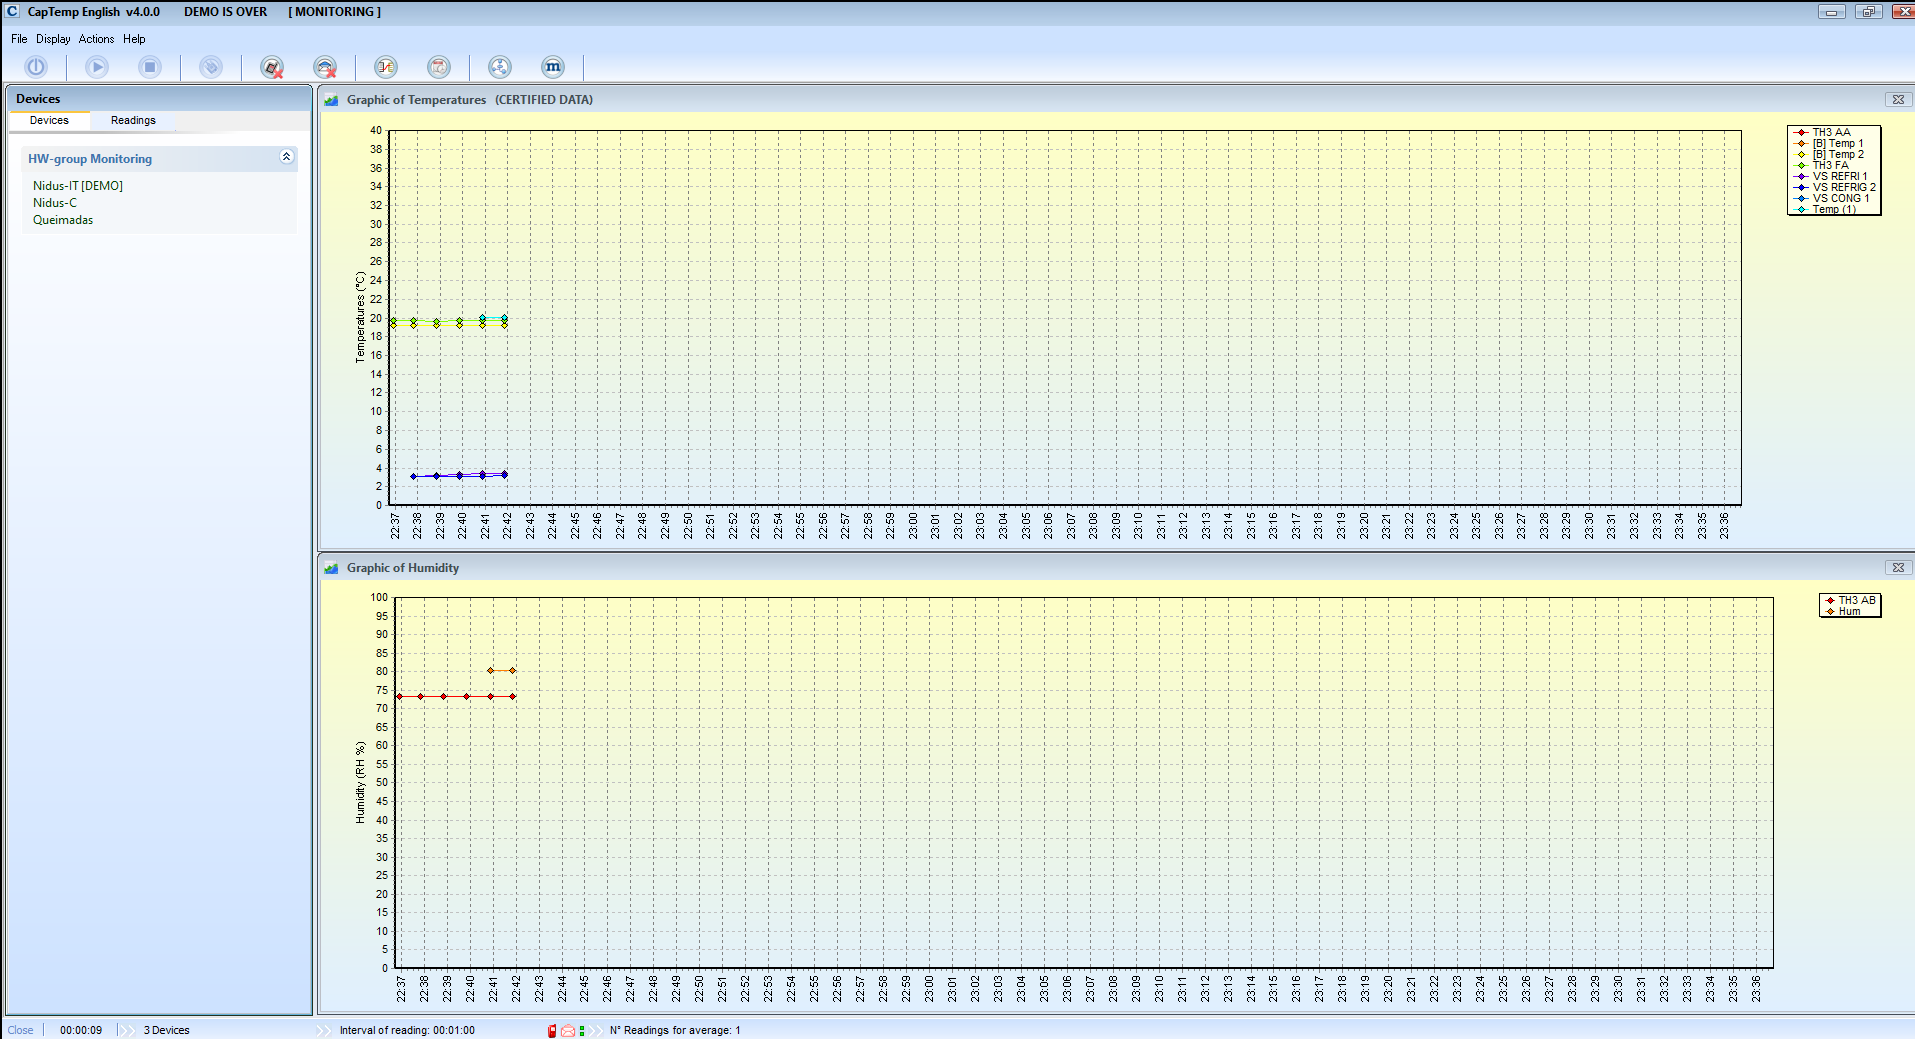
\includegraphics[width=1.00\textwidth]{images/captemp.png}
  \caption{CapTemp SQL}\label{figcaptempsql}
\end{figure}
O registador desenvolvido pela Captemp, representado na figura \ref{fignidusCl} denomina-se por Nidus-C, um registador que suporta até 32 sensores.\par

\begin{figure}[ht]
  \centering
  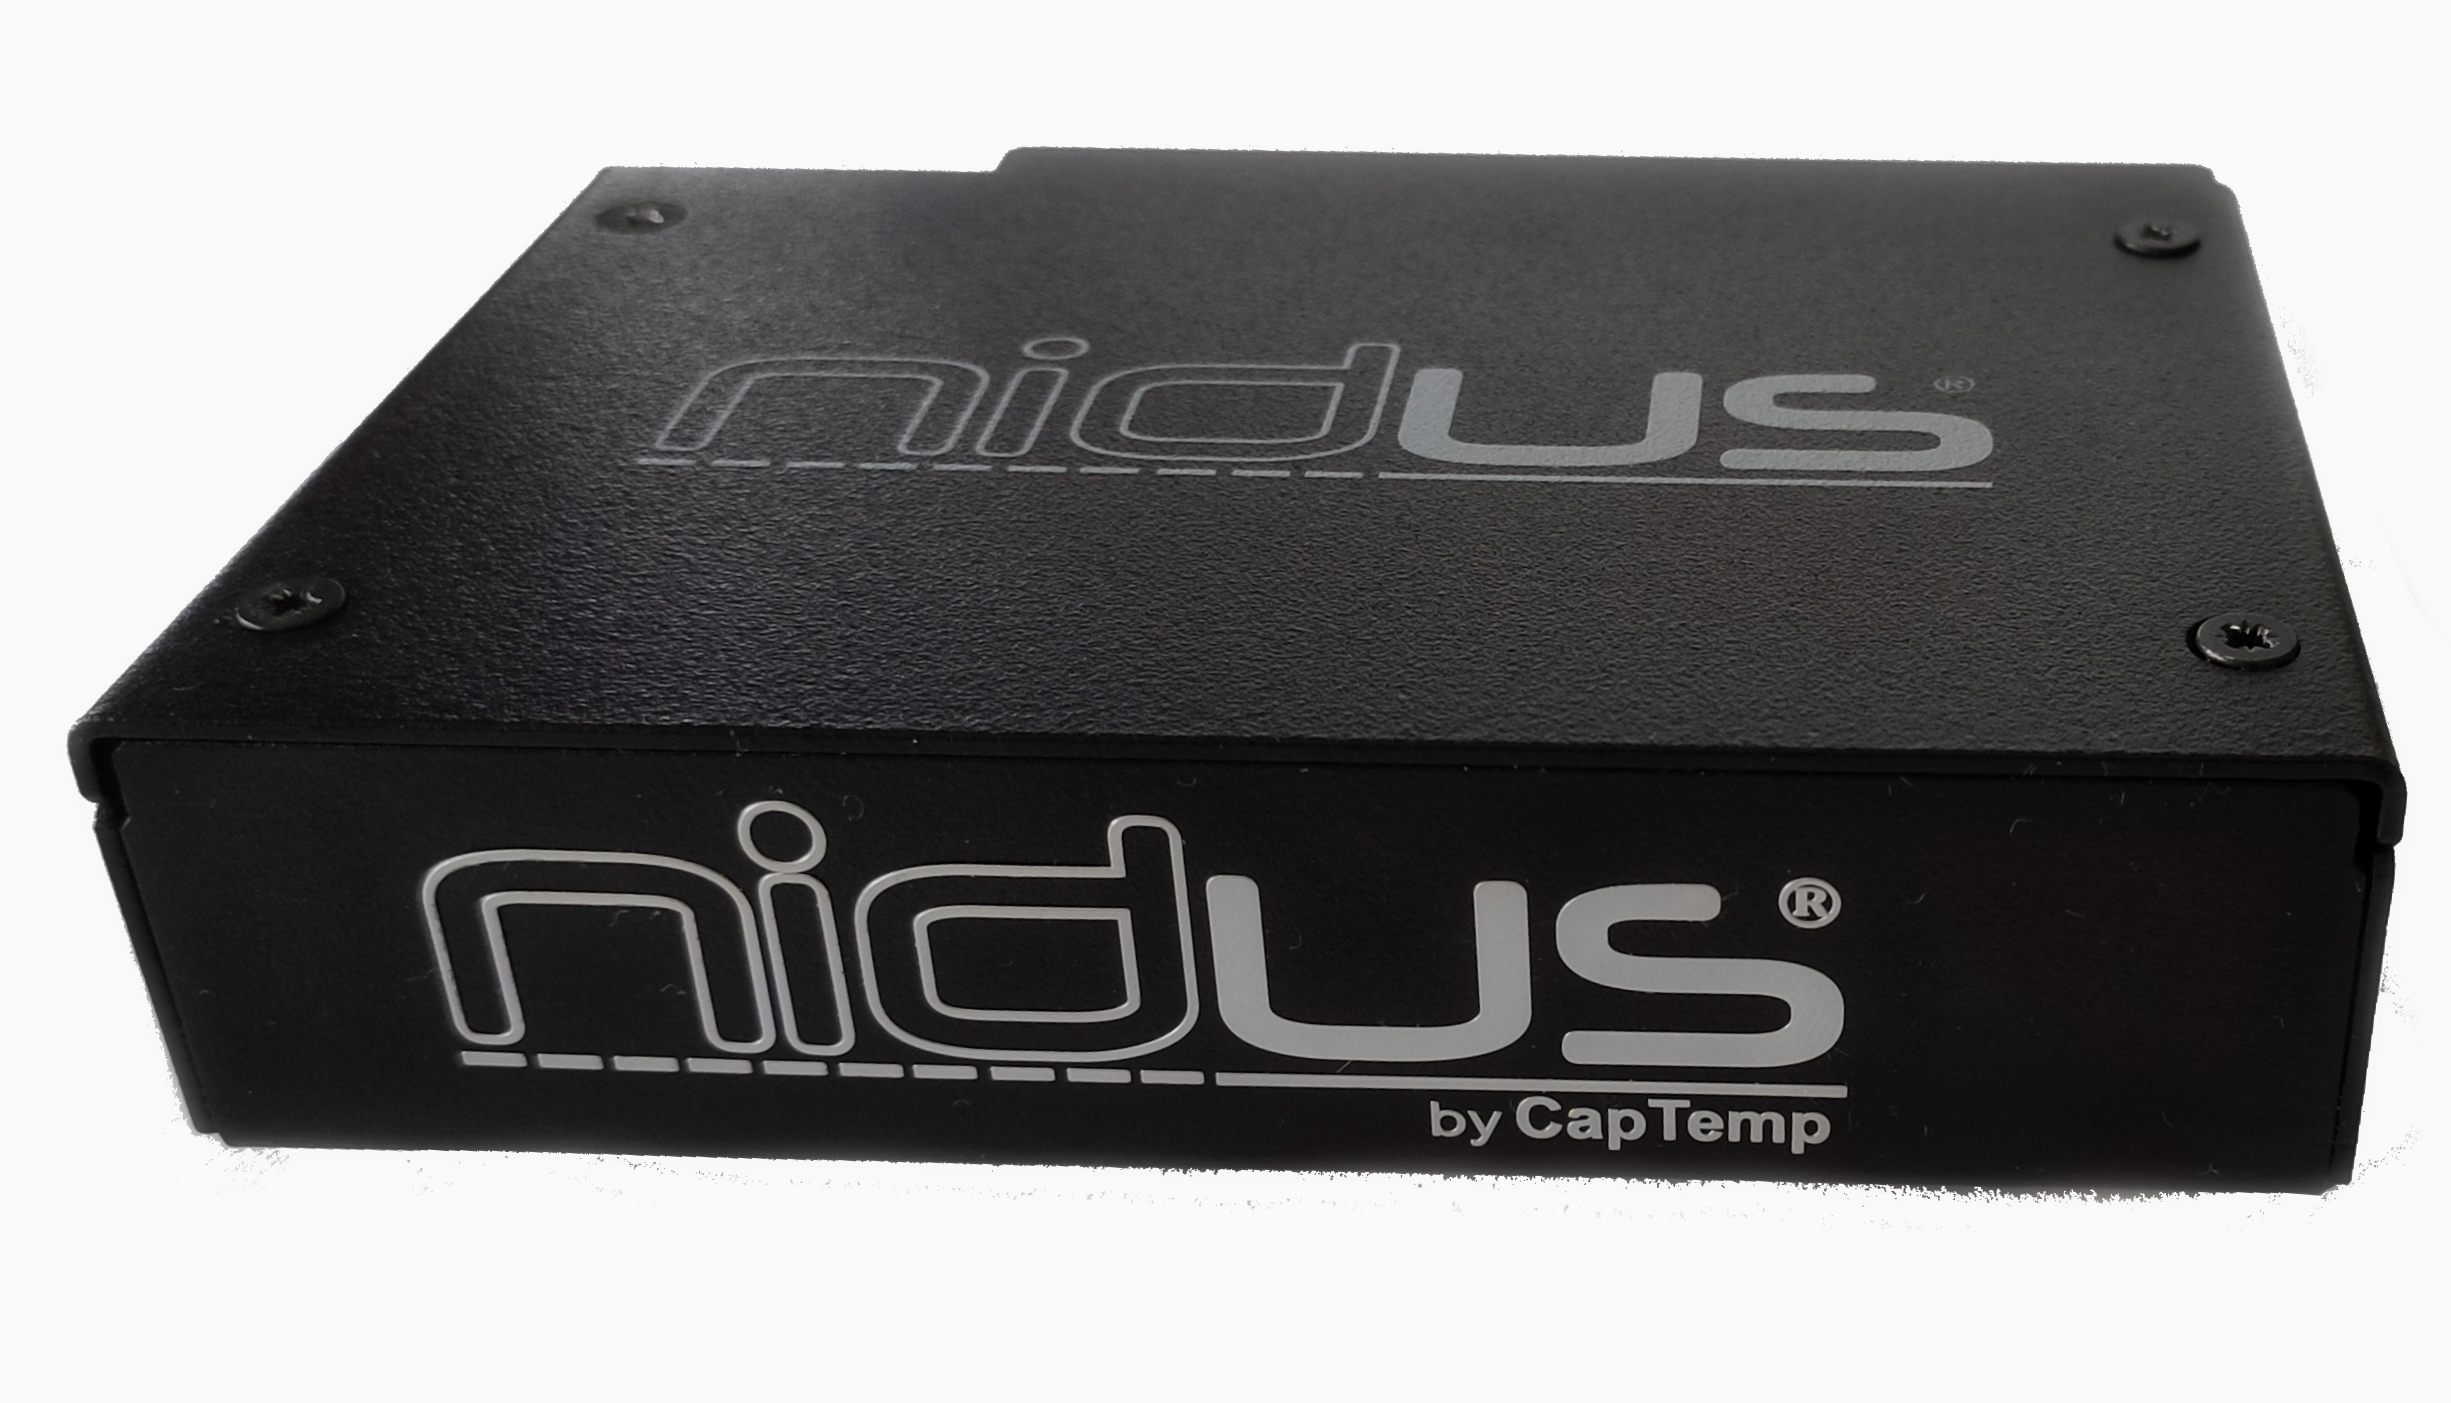
\includegraphics[width=0.45\textwidth]{images/nidus.jpg}
  \caption{Coletor de dados Nidus-C}\label{fignidusCl}
\end{figure}

Com a necessidade de mais funcionalidades, a Captemp criou diversas variantes da Nidus-C, representadas na Figura \ref{fignidusall} para aplicar em outras áreas para além da Meteorologia Legal. Das quais surgiram a Nidus-C+, uma versão similar da Nidus-C acrescentando a possibilidade de adicionar sensores \textit{Wireless}. A Nidus-IT e Nidus-IT+ duas versões com as funcionalidades da Nidus-C e Nidus-C+ respetivamente, acrescentando Inputs e Outputs ao sistema de monitorização. Para soluções exclusivamente \textit{Wireless} nasce a Nidus-W suportando apenas sensores Wireless. Por último é desenvolvido a Nidus-R, baseada na Nidus-IT especialmente desenhada a pensar em ambientes IT com suporte para montagem em bastidores.
\par
\begin{figure}[ht]
  \centering
  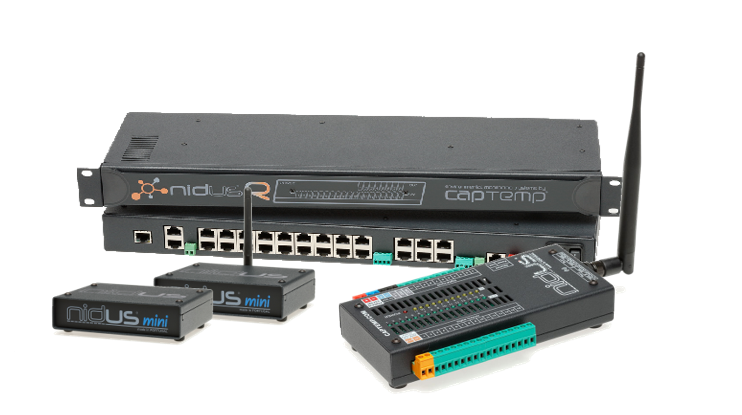
\includegraphics[width=0.65\textwidth]{images/nidusall.png}
  \caption{Universo Nidus}\label{fignidusall}
\end{figure}

No setor dos sensores foi desenvolvido o TH3, um conversor RS485 permitindo às diversas Nidus, ligar por RS485 a sensores 1Wire além dos dois inputs possuídos no TH3. Nos sensores \textit{Wireless}, foi desenvolvido o Airo à semelhança do TH3 possui dois inputs, um ecrã e possibilita a ligação de sensores 1Wire. Permite ainda a leitura de todos os Airo adicionados na Nidus ao mesmo tempo, tecnologia desenvolvida pela Captemp denominada por Captemp AST \cite{Captemp_AST}. Ambos os sensores estão representados na Figura \ref{figairoth3} 
\begin{figure}[ht]
  \centering
  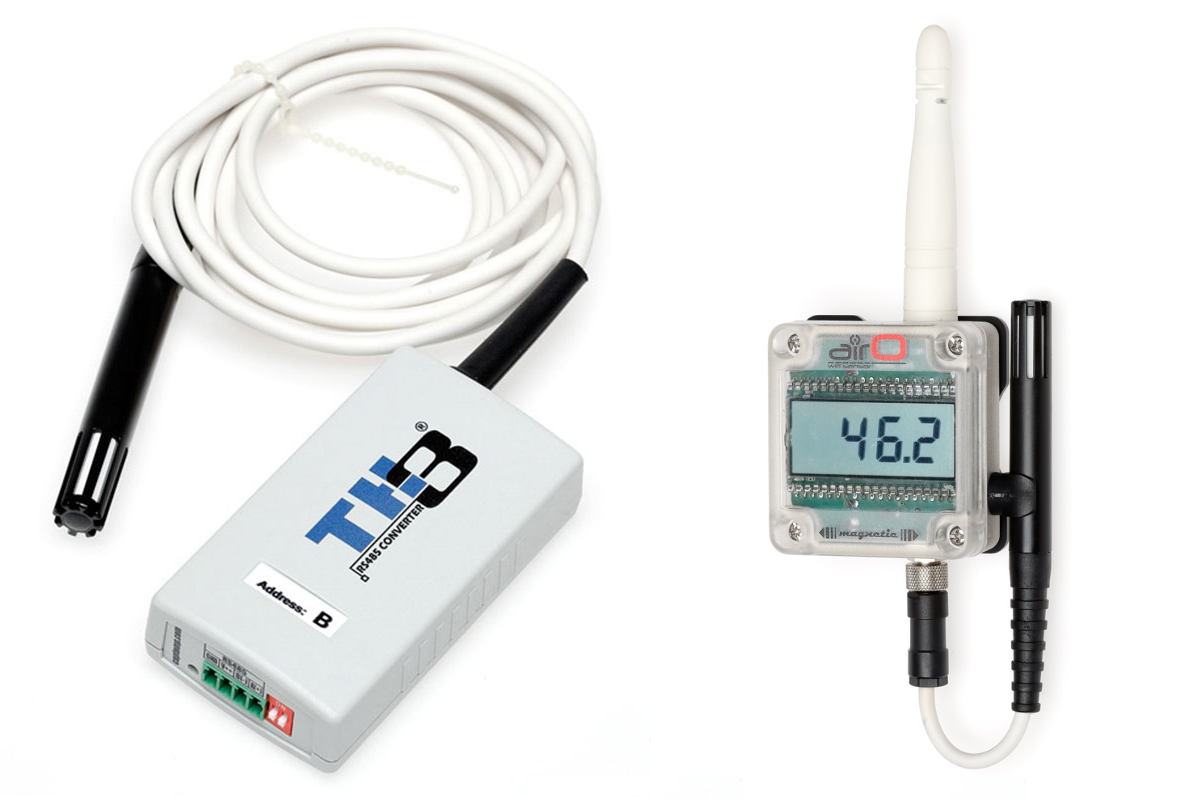
\includegraphics[width=0.45\textwidth]{images/th3airo.png}
  \caption{ TH3 e Airo}\label{figairoth3}
\end{figure}
\par
Em desenvolvimento encontram-se sensores com recurso a tecnologias NB-Iot, Beacon's BLE e Lora entre outras soluções tais como sistemas de rastreamento de Febre em tempo real com recurso a inteligência artificial.
\par
A Captemp desenvolve igualmente um portal \textit{Cloud} denominado Senslive (Figura \ref{figsenslive}) que possibilita a centralização dos sistemas de monitorização numa única plataforma \textit{Cloud}.

\begin{figure}[ht]
  \centering
  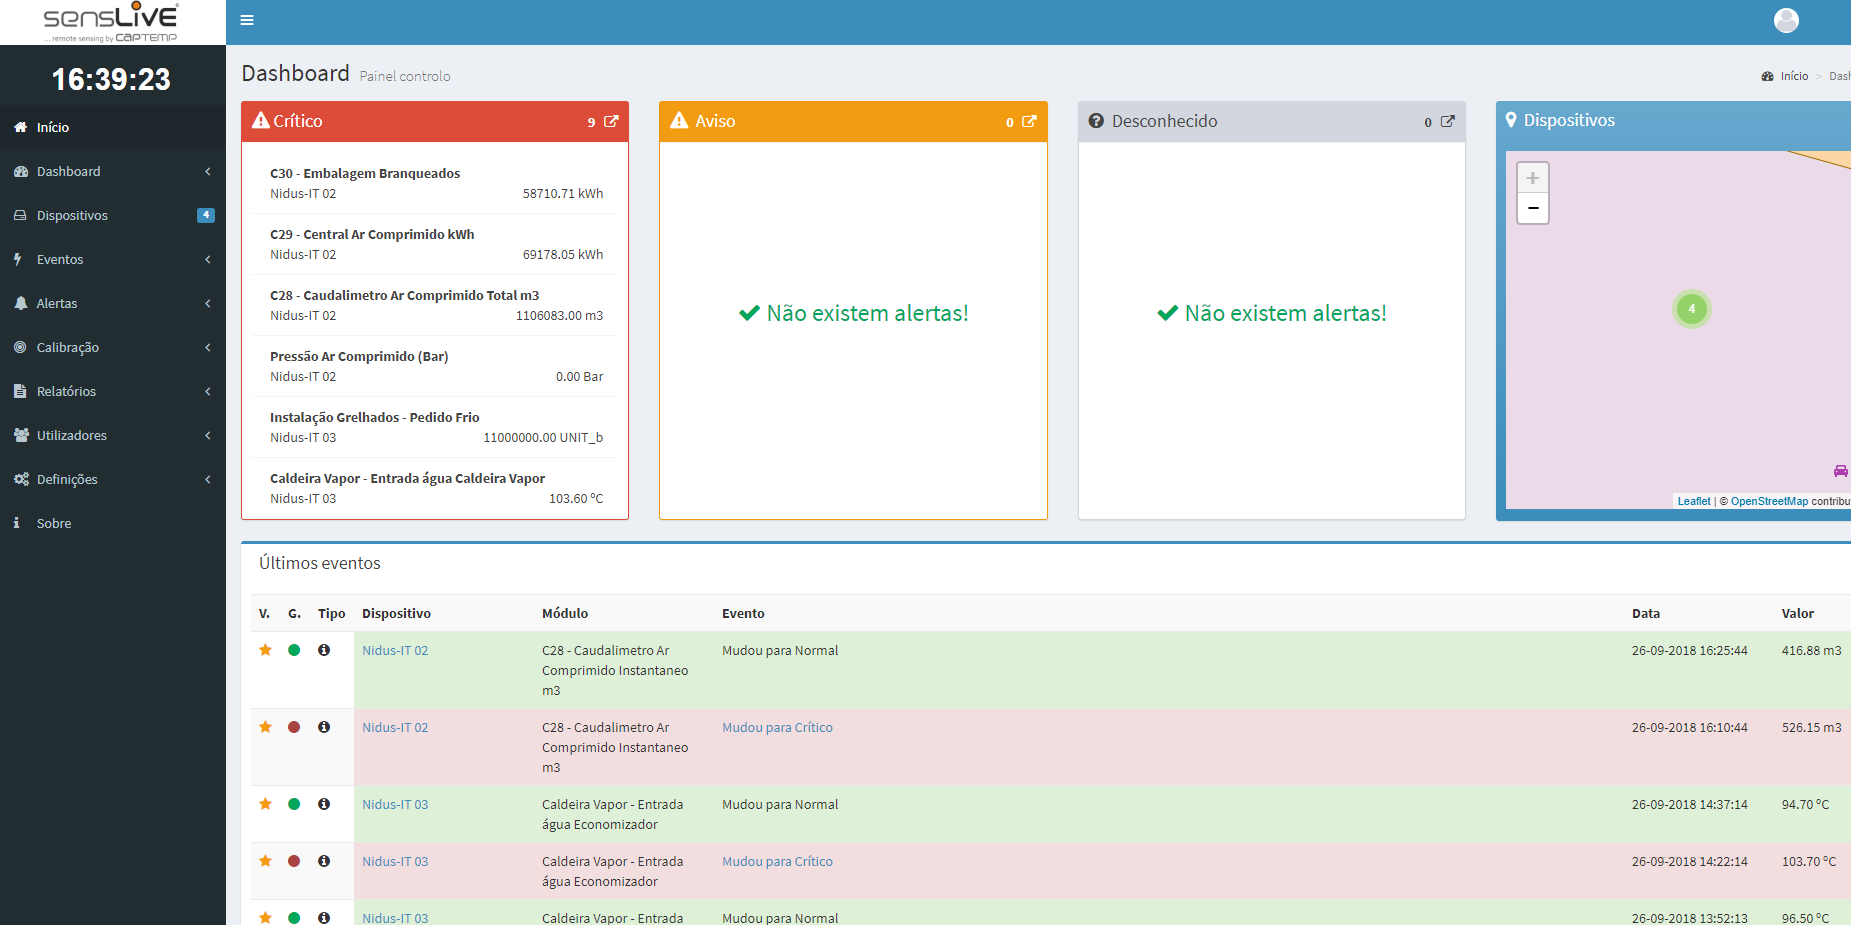
\includegraphics[width=0.95\textwidth]{images/mwsnap0791.png}
  \caption{ Portal Senslive}\label{figsenslive}
\end{figure}



\section{Motivação e Objetivos}
\par
O estágio é uma forma do estudante colocar numa situação de contexto profissional os conceitos adquiridos em contexto académico. A realização de um estágio é também uma mais valia pois possibilita o adquirir de experiência profissional que não é possível obter em contexto escolar.
\par
A Captemp com os projetos a desenvolver pretende melhorar constantemente os seus equipamentos e as suas interfaces, por questões de \textit{Markting} quer pelo próprio evoluir da tecnologia e necessidade de novas funcionalidades e o seu desenvolvimento requer o alojamento de mais recursos como por exemplo a memória ou disco, estes limitados nestes tipos de equipamentos e onde é preciso fazer uma correta escolha de soluções e de implementação. 
\par
Ao longo do estágio, o objetivo será estudar variados mecanismos que permitam adotar recursos web modernos nos equipamentos de baixos recursos. Serão aplicados vários conhecimentos adquiridos durante o percurso académico de modo a melhorar a interface para o utilizador, técnicas de otimização de código, compressão de ficheiros, manipulação de imagens de modo a ocupar o mínimo de espaço permitindo futuros desenvolvimento e melhorias, dando continuidade ao suporte do projeto Nidus. Igualmente serão criados três novos projetos de desenvolvimento de novos equipamentos e soluções que tiram partido de novas tecnologias como o NB-Iot e Beacon’s BLE onde é necessário devido á escassez de recursos fazer a correta gestão dos mesmos e a implementação de variados algoritmos.
\par
Nas seguintes secções são apresentadas uma breve descrição de cada projeto, dos equipamentos já existente e desenvolvido, e as funcionalidades a desenvolver em cada projeto.
\subsection{Nidus}
\par
O projeto "Nidus" tem como objetivo dar suporte ao \textit{Front-end} das Nidus já existentes para correções de bugs encontrados em versões anteriores, otimização de código, de modo a ocupar o mínimo espaço, possibilitando deixar memória livre para desenvolvimentos futuros, desenvolver versões customizadas com \textit{layouts} a pedido do cliente com funcionalidades especificas, ou simplesmente melhorar a página seguindo a tendência de equipamentos concorrentes.
\subsection{NB-Iot}
Com o surgimento da nova tecnologia NB-Iot surgiu a necessidade de serem criados equipamentos que tirem partido dessa tecnologia e as suas vantagens. Para tal durante o estágio será desenvolvido um dos equipamentos que tira partido da tecnologia. Este projeto tem como por objetivo criar uma versão de raiz, simplificada e mais barata de um outro equipamento de NB-Iot em desenvolvimento pela Captemp, através do módulo Xbee da DIGI e da sua programação em Micropython. Durante o projeto será necessário garantir a correta gestão de memória, gestão de Logs internos, comunicação com os sensores físicos, comunicação bidirecional e encriptação com o portal Senslive.
\subsection{Kea Tracker}
O "Kea Tracker" é um projeto de Beacon’s BLE que comunicam com o \textit{smartphone}, onde é possível definir alertas locais no \textit{smartphone} e envio dos dados obtidos dos sensores das beacon’s e envio para a plataforma Senslive.
Tal como o projeto anterior será necessário além de criar uma aplicação para \textit{smartphone}, criar \textit{Firmware} específico para as beacon’s que na ausência de comunicação com o \textit{smartphone} devem armazenar em Log as leituras dos sensores e quando este está ao alcance descarregar para o \textit{smartphone}.
\subsection{dot.Tracker}
A pedido de um cliente foi solicitado o desenvolvimento de uma plataforma para localização de pessoas e objetos em ambientes \textit{inndoor}. O cliente pretende ter uma plataforma onde seja capaz de ver em tempo real a posição de pessoas e objetos definidos previamente, definir zonas de alerta, e consultar o histórico de movimentos. Neste projeto irão ser usadas beacon's BLE e vários \textit{Gateways} BLE estrategicamente colocados no edifício e responsáveis por receber o \textit{broadcast} das beacons que por sua vez transmitem para o servidor através da rede informática do cliente do serviço. O projeto é constituído pelo desenvolvimento da plataforma de gestão e visualização, pelo recetor dos pacotes provenientes dos equipamentos e respetivos cálculos segundo o algoritmo a adotar.

\section{Problemas identificados}
Foram identificados diversos problemas em cada um dos projetos a desenvolver durante o estágio. Uma breve descrição é apresentada de seguida.
\par
A página WEB da Nidus desde a sua criação já sofreu muitas alterações para seguir os padrões e tendências da concorrência e, portanto, está em constante atualização. Atualmente com a mundialização quase todas as pessoas sabem inglês, mas existem algumas pessoas que ou não sabem ou preferem usar a língua nativa. Para tal a Captemp pretende desenvolver uma página WEB com um sistema de tradução e diversas línguas que seja possível de alojar na memória do equipamento, devido aos problemas já referidos para o utilizador escolher a linguagem e assim cativar mais clientes e expandir a Captemp para outros países. Com o acréscimo do serviço de internalização surge o problema de uma interface com necessidade de mais armazenamento. Terão de ser estudadas otimizações que se possam implementar no código já existente. Existe a necessidade de estudar o melhor método de compressão da página mantendo o GZIP utilizado atualmente ou migrar para outro mais recente como o Brotli e a compressão de imagens migrando as imagens existentes para imagens SVG, possibilitando outras soluções para a página com sistemas mais interativos e ocupando o menor espaço disponível. Além dos problemas referidos anteriormente poderão surgir novas funcionalidades, a pedido de clientes, como por exemplo páginas com layout específicos ou novos sensores e a simples correção de possíveis Bugs encontrados.
\par
Outro problema a resolver detetado pelo \textit{feedback} recebido dos clientes é a complexidade para a criação de eventos, ações e reações, que controlam o Sistema Nidus. Para isso a Captemp pretende reformular a estrutura de gestão de eventos para um sistema mais visual e atual similar ao Scratch, um \textit{software} utilizado atualmente para ensinar a crianças as bases da programação e elas mesmos criarem alguns programas sem saber nenhuma linguagem de programação. Na figura \ref{scratch} é apresentado um exemplo de programação usando a ferramenta Scratch, onde o utilizador com um sistema de blocos pode criar condições e eventos a despoletar consoante algumas condições.

\begin{figure}[ht]
  \centering
  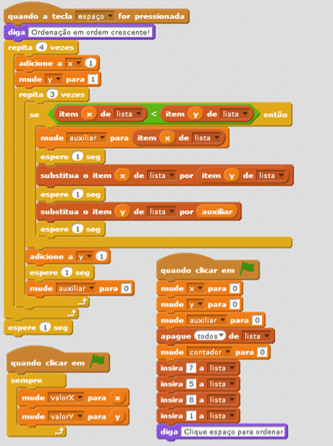
\includegraphics[width=0.50\textwidth]{images/scratch.png}
  \caption{ Programação com a ferramenta Scratch}\label{scratch}
\end{figure}

\par Outros problemas existentes, a resolver durante o estágio, são a criação de sistemas \textit{low-cost}, de outros equipamentos CapTemp, para clientes que não necessitem de tantas funcionalidades com a introdução da alternativa para NB-Iot com recurso ao módulo Xbee da Digi, e a substituição de produtos antigos descontinuados, os data-logger(Figura \ref{ds1921}) e sua substituição por similares com as mesmas funções e mais tipos de sensores disponíveis, uma necessidade também já requisitada pelos clientes que pretendem monitorizar mais grandezas além da temperatura, mas com os padrões e tecnologias dos dias de hoje e com suporte para o novo Portal da Captemp o Senslive. Ou simplesmente o desenvolvimento de novos produtos a pedido dos clientes.

\begin{figure}[htb]
  \centering
  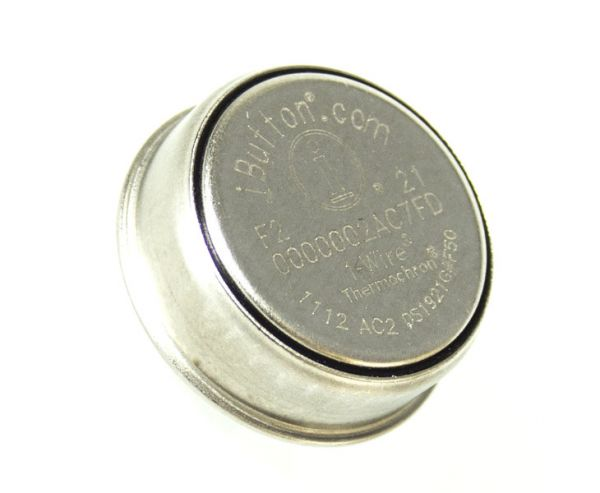
\includegraphics[width=0.20\textwidth]{images/ds1921.jpg}
  \caption{Data Logger iButton}\label{ds1921}
\end{figure}


\par
Em resumo os problemas a solucionar durante o estágio podem ser encontrados na seguinte lista:
\begin{itemize}
\item Melhorar a compressão da página WEB da Nidus;
\item Melhorar a compressão das imagens presentes na página WEB da Nidus;
\item Correção de Bugs da página Web da Nidus;
\item Melhorar o processo de criação de eventos;
\item Criação de uma página com sistema de tradução automático;
\item Versões customizadas da página WEB a pedido do cliente;
\item Seguir as tendências da concorrência;
\item Criação de soluções/equipamentos de baixo custo;
\item Substituição de produtos descontinuados;
\item Desenvolvimento de produtos à medida do cliente.

\end{itemize}

\section{Organização do relatório}

\par Este presente relatório está dividido em 5 capítulos. O primeiro capítulo faz a introdução ao tema e é apresentado os objetivos, o enquadramento do estágio e alguns aspetos inicias a considerar. 
\par No capítulo seguinte é apresentada a tecnologia e hardware pesquisado com fim a dar suporte a este mesmo estágio e uma pequena pesquisa sobre projetos/produtos similares quer na finalidade quer nas tecnologias usadas e o estado atual de cada projeto. 
\par O capítulo 3 apresenta o trabalho desenvolvido durante o estágio na empresa para a resolução dos problemas identificados. Este capítulo apresenta os detalhes técnicos das soluções escolhidas. 
\par No capítulo 4 são descritos os resultados dos testes efetuados às soluções propostas e desenvolvidas no capítulo 3.
\par Por fim no capítulo 5 é apresentada uma breve conclusão de todo o trabalho, dificuldades e algumas sugestões para futuras implementações. 


	% Arabic numbering starts

% For each chapter, you should have a bit of code that looks like this:
% \label allows you to later \ref that chapter.
% \input includes a different .tex file, so that you can have you dissertation
% neatly partitioned into several files. I recommend one file per chapter.
\chapter{Estado da Arte}
\label{chap:state_of_the_art}

\section{Introdução}
Nesta secção é apresentada o estado da arte dos projetos realizados durante o estágio na empresa CapTemp. Nessa ordem é apresentado o funcionamento do sistema do Nidus desenvolvido pela empresa CapTemp e a sua página de configuração e visualização. Na secção \ref{Página do Coletor de Dados Nidus} são apresentadas também as metodologias e tecnologias que o sistema implementa atualmente para a compressão das páginas que dão suporte ao sistema. Na secção \ref{nbiot}, \ref{kea} e  \ref{dot} irá ser introduzido o plano inicial dos projetos a desenvolver e a base já existente tal como as tecnologias que estes irão utilizar. Na secção \ref{solucoesDisponiveis} será abordado as soluções e tecnologias existentes na comunidade científica e alguns produtos similares, já existentes para os projetos anteriormente referidos.

\section{Coletor de Dados - Nidus} \label{Coletor de Dados - Nidus}
\par
O sistema Nidus, apesar das suas diversas versões de hardware partilha entre todas as versões o mesmo centro de processamento o módulo RCM6760 da Rabbit. O sistema Nidus é composto por dois módulos principais, o Back-end que gere toda a parte de leitura de sensores, de atuação e envio de alertas, log entre as demais funcionalidades e o Front-end, duas páginas WEB Single-Application de modo a não sobrecarregar o módulo com a interface e mover o processamento da interface para o browser do cliente. Na primeira página é possível visualizar os valores obtidos pelo Back-end com atualização em tempo real. Na segunda página e possível carregar as configurações para realizar alterações nas mesmas. A comunicação entre os dois componentes é feita através de XML. Para consultar os valores na primeira página o Front-end acede ao ficheiro values.xml gerado pelo Back-end onde contém todas os valores necessários. Na página de configurações á semelhança da primeira página os valores são carregados por um ficheiro XML o ficheiro setup.xml, incluindo a particularidade de aceitar pedidos POST de modo a alterar as configurações do equipamento.
\par A Nidus dispõe de base para o utilizador variadas funcionalidades tais como, leitura de sensores TH3 e Airo, INPUTS digitais, OUTPUTS digitais e analógico, leitura de sensores SNMP e MODBUS, envio de alertas via GSM e E-mail, programação de eventos, envio automático para um portal Cloud e Log Interno. Outras funcionalidades estão disponíveis mediante o pedido do cliente tais como sensores específicos, leitura de sensores por RS232 ou protocolos de comunicação específicos.
Na tabela \ref{tab0} são apresentadas as principais características do módulo RCM6760 da Rabbit.




\begin{table}[htb]
\centering
\caption{Especificações do Módulo RCM6760}\label{tab0}
\begin{tabular}{|c|c|}\hline
Microprocessor&Rabbit 6000 \\\hline
Frequencia do Microprocessor &200 MHz\\\hline
Flash Memory &4 MB (Código e Sistema de Ficheiros)\\\hline
SRAM&1 MB\\\hline
Power &260 mA 3.3V - Ethernet ON\\\hline
\end{tabular} 
\end{table}

\subsection{Páginas do Coletor de Dados Nidus} \label{Página do Coletor de Dados Nidus}
\par
O código desenvolvido de modo a chegar á fase de produção é comprimido e compilado de modo a que ocupe o mínimo espaço e possa ser armazenado na memória do módulo e coabitar com o Firmware de Back-end, segue os seguintes passos de desenvolvimento:
\begin{enumerate}
\item Desenvolvimento/ alteração do código JavaScript necessário; 
\item Compressão das Imagens necessárias com recurso a ferramentas online tais como o TinyPNG\cite{tinypng} e posterior conversão em Base64 para incluir no JavaScript a imagem e o mesmo poder fazer a gestão da apresentação
\item Compilação/compressão do JavaScript num ficheiro único com recurso ao Google Clousure Platform, nesta etapa para cada versão de hardware é compilado consoante os ficheiros a incluir, poupando o espaço não necessário como o código referente aos Inputs e Outputs na Nidus C, C+ e W, ou o código referente ao módulo wireless nas versões não Wireless.
\item Geração do minificado do código HTML
\item Compressão de cada ficheiro para o seu respetivo GZIP
\end{enumerate}
\par
Após estes passos fica disponível uma nova versão da página pronta a ser carregada na Nidus.
Na imagem \ref{fignidusPage} é apresentado o estado e layout de uma página da Nidus IT no momento do início do estágio.

\begin{figure}[ht]
\centering
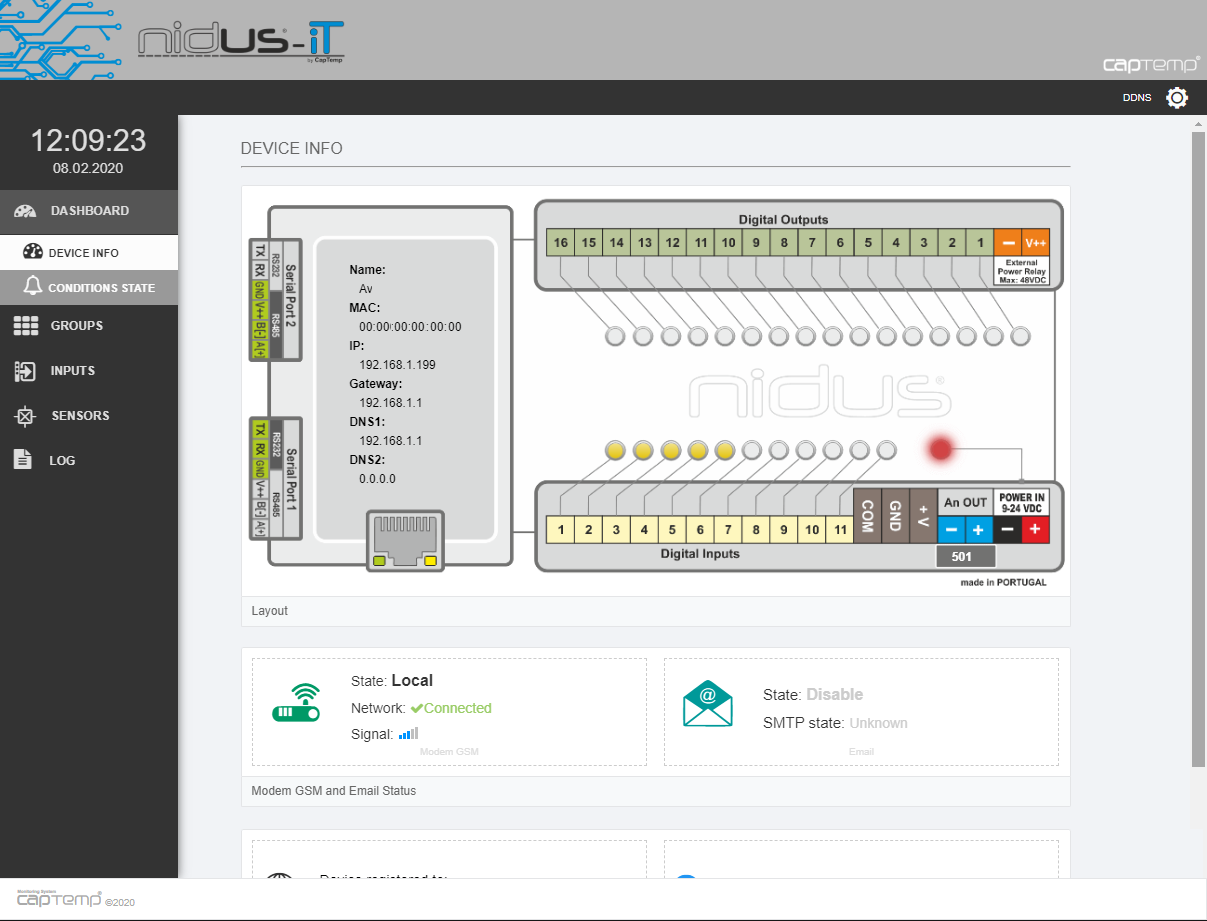
\includegraphics[width=0.75\textwidth]{images/layoutPAginaInit.png}
\caption{Layout página da Nidus IT no início do estágio}\label{fignidusPage}
\end{figure}


\section {NB-Iot \& Digi Xbee 3 }\label{nbiot}
\par
Os módulos Xbee 3 representado na figura \ref{figxbee} da DIGI dispõe recentemente de uma versão NB-Iot/ LTE. Ideal para projetos com baixo volume de transmissão de dados e com baixo consumo de energia. O módulo inclui também um compilador de Micropython, contundo a versão Micropython desenvolvida pela DIGI e incluída no módulo XBee, não inclui todas as funcionalidades do Micropyhton tais como por exemplo a biblioteca de gestão de Arrays e o módulo de "\_thread" pois o mesmo não tem suporte para multithread.
Na tabela \ref{tab1} são apresentadas as principais características do módulo XBee 3 da Digi\cite{Digixbee}.

\begin{figure}[ht]
\centering
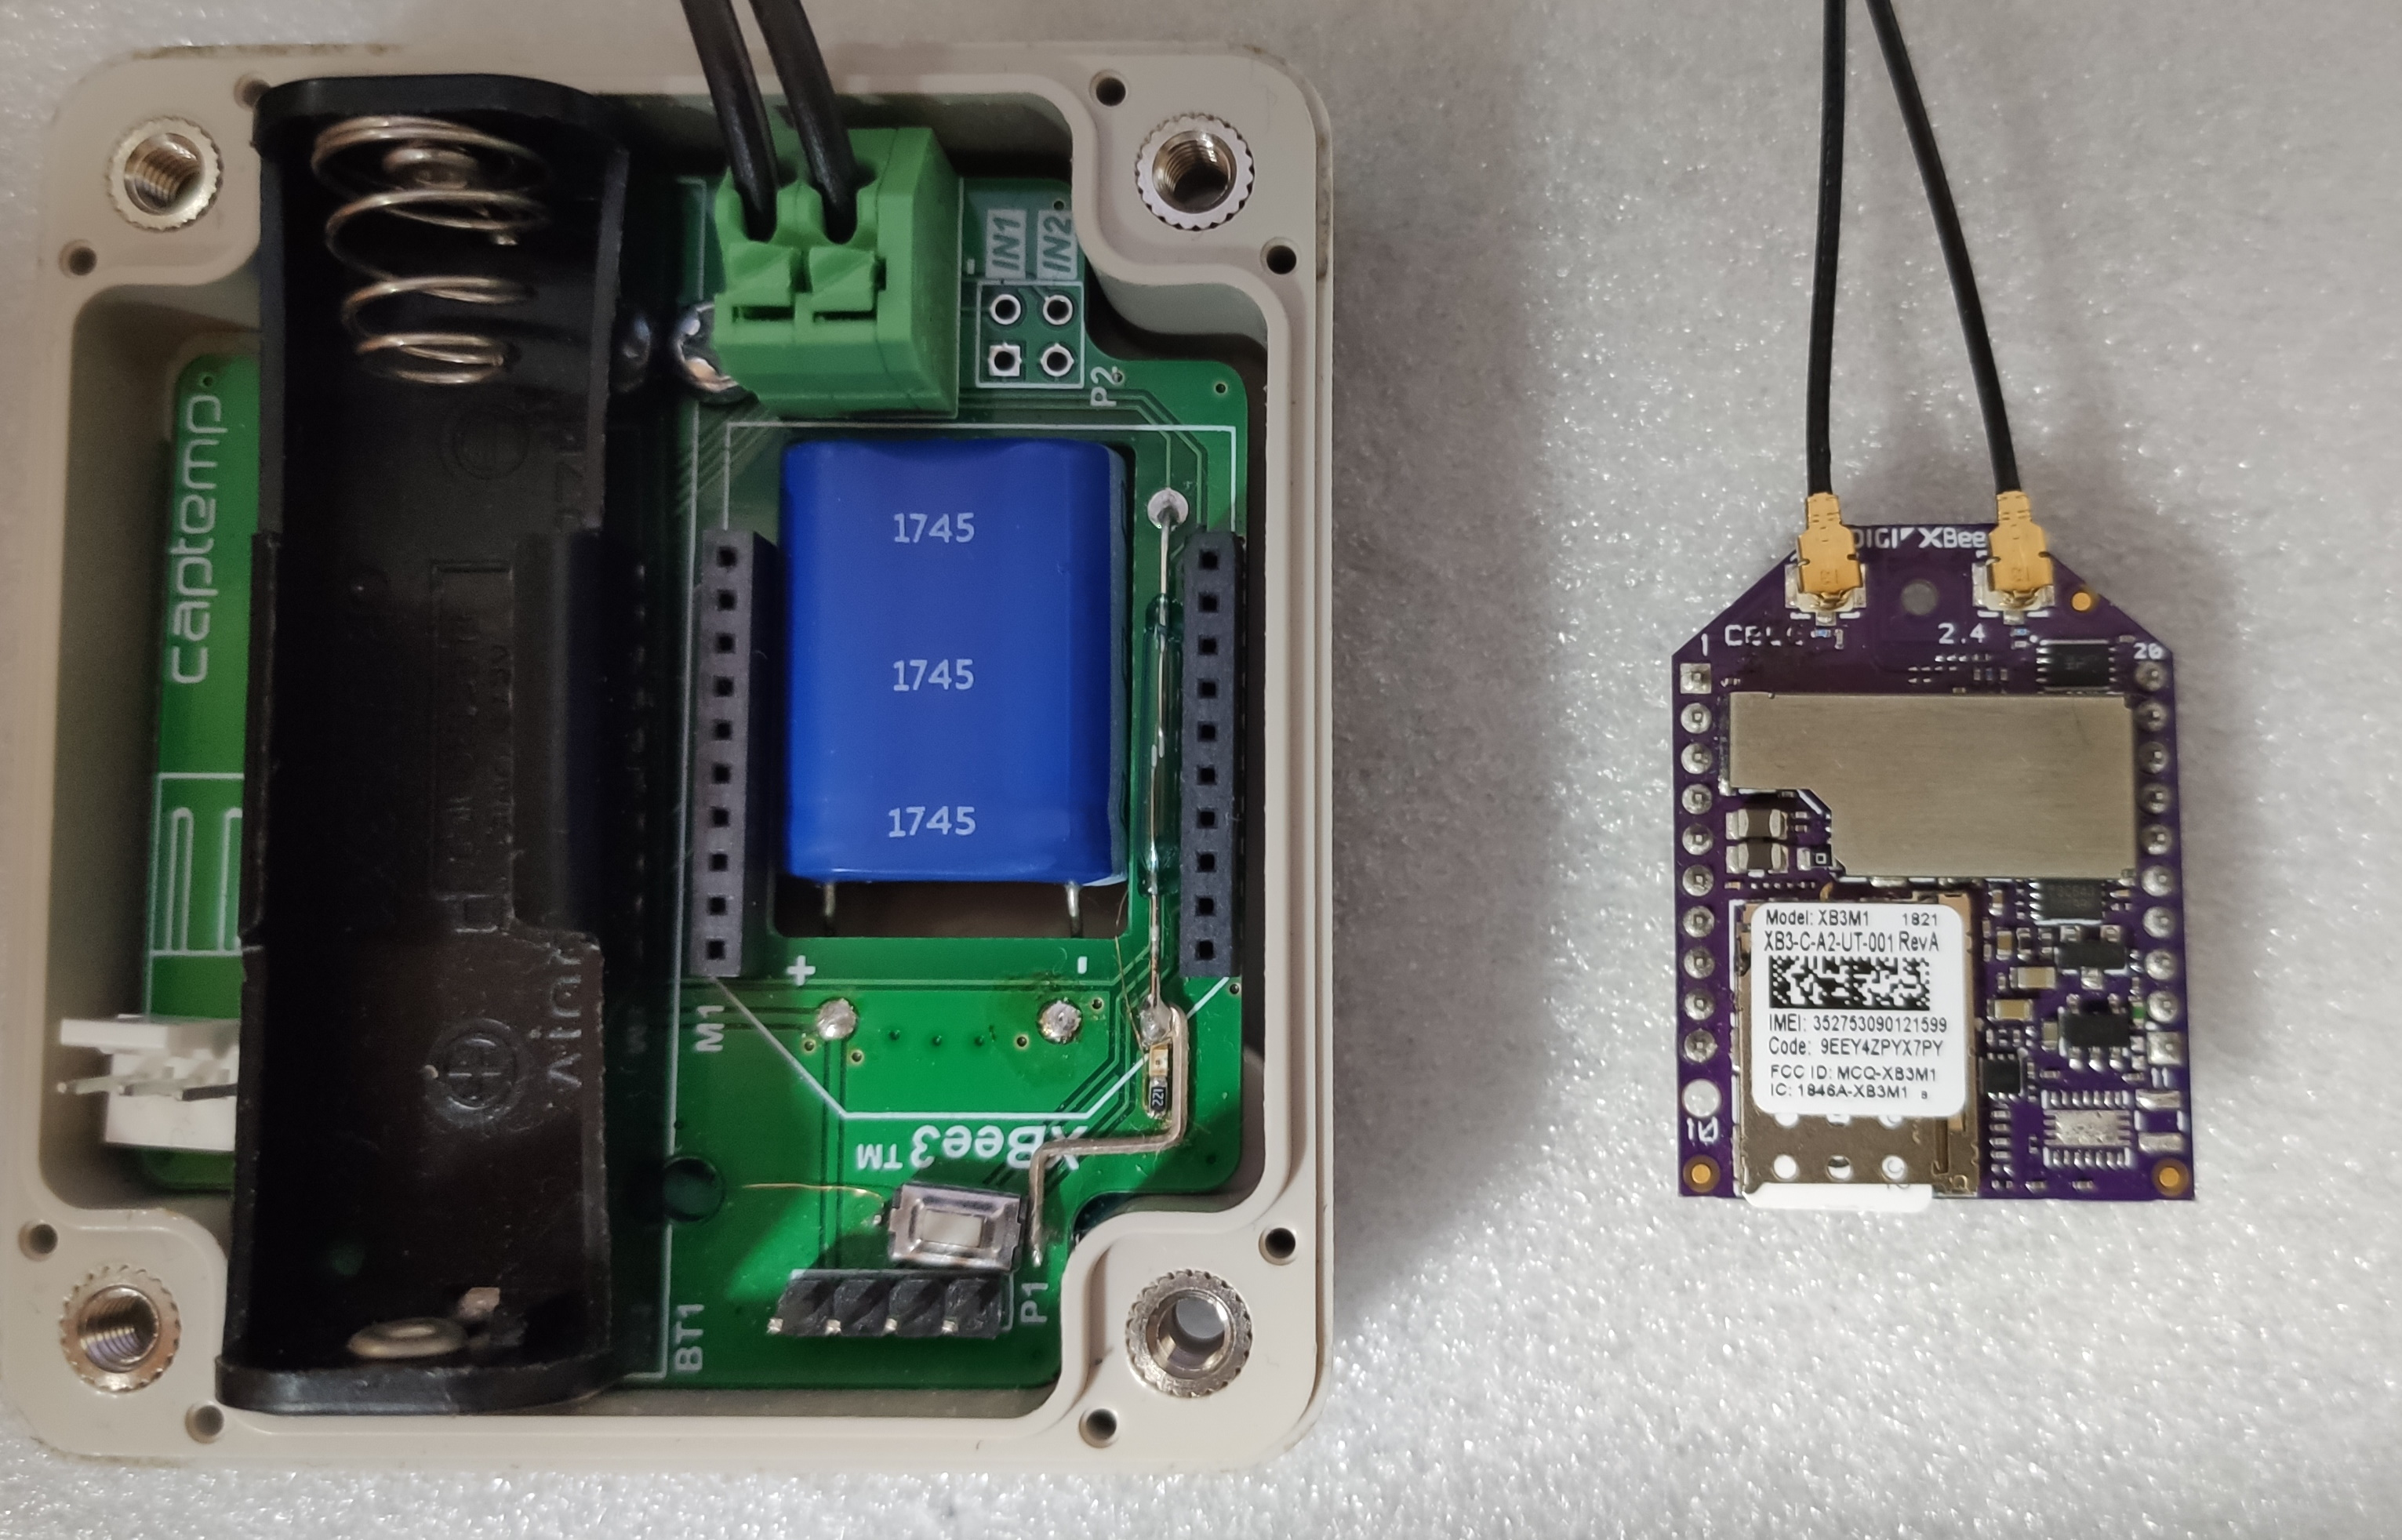
\includegraphics[width=0.60\textwidth]{images/xbee.jpg}
\caption{Módulo Xbee 3 e placa de expansão desenvolvida pela Captemp}\label{figxbee}
\end{figure}

\begin{table}[htb]
\caption{Especificações do Módulo Xbee 3}\label{tab1}
\begin{tabular}{|c|c|}\hline
Chipset& U-blox SARA-R410M-02B\\\hline
Dimensões& 24.38 mm x 32.94 mm \\\hline 
Temperatura de Funcionamento& -40º C to +85º C \\\hline 
Tipo de SIM & 4FF Nano \\\hline
Interfaces& UART, SPI, USB \\\hline 
Programação MicroPython& 32 KB Flash / 32 KB RAM \\\hline 
I/O& 4 ADC (10-bit), 13 I/O digitais, USB, I2C \\\hline 
Bluetooth& BLE Ready \\\hline 
Potencia de Transmissão& Até 23 dBm \\\hline 
Sensibilidade de Receção (LTE-M) & -105 dBm \\\hline 
Sensibilidade de Receção (NB-IoT) & -113 dBm \\\hline 
Velocidade Downlink/Uplink(LTE-M) & Até 375 kb/s \\\hline 
Velocidade Downlink/Uplink(NB-IoT) & Até 27.2 kb/s Downlink, 62.5kb/s Uplink \\\hline 
Alimentação & 3.3-4.3VDC \\\hline 
Pico corrente na transmissão & \begin{tabular}{@{}c@{}} 550mA - Bluetooth OFF \\ 610mA - Bluetooth ON\end{tabular}\\\hline 
Corrente média de transmissão (LTE-M) & 235mA \\\hline 
Corrente média de transmissão (NB-IoT) & 190mA \\\hline 
Modo Power Save& 20uA \\\hline 
Modo Deep Sleep& 10uA \\\hline 
\end{tabular} 
\end{table}

\par A Captemp pretende, através da utilização deste módulo e de uma placa de expansão desenvolvida pela própria, apresentada anteriormente na figura \ref{figxbee}, desenvolver uma versão do seu outro equipamento de Nb-Iot, mais simples representando numa opção de menor custo para o cliente. Será necessário desenvolver todo o código referente à gestão interna de Logs para guardar informação quando não existe cobertura para envio, o agendamento do envio e leituras, otimização da memória e bateria e implementação de comunicação bidirecional com encriptação com o portal Senslive. Sempre com recurso á programação em MicroPython.
A placa de expansão inclui um módulo de RTC, um conversor 1Wire para possibilitar a leitura de sondas já desenvolvidas pela Captemp, um sistema de alimentação para possibilitar a alimentação por pilha ou por alimentação externa. Ao desenvolver todo o equipamento a empresa tem o controlo total sobre o Firmware e sobre a estrutura de envio e a vantagem de tornar o equipamento compatível com todos os sensores que já possui.

\subsection {MicroPython}
\par O MicroPython\cite{MicroPython}, lançado em 2014, é um compilador e interpretador que implementa a linguagem Python3 e otimiza o seu funcionamento em microcontroladores. Escrito em C e disponibilizado em Open-Source é possível adaptar o mesmo para os diversos equipamentos. \par
É suportado por diversas arquiteturas de processadores tais como:
\par
\begin{itemize}
\item x86
\item x86-64
\item ARM
\item ARM Thumb
\item Xtensa
\end{itemize}
\par
Em microcontroladores que suportem Multi-thread , não sendo o caso do módulo usado está disponível ao programador o módulo de "\_thread" para criar processamento paralelo. Disponibiliza a programação de interrupções físicas, uteis em microcontroladores, tem disponível um "Garbage collector" para gerir a memória do microcontrolador e bibliotecas tais como "usocket" para criação e gestão de sockets, "network" para gerir a comunicação com o módulo específico de cada microcontrolador, ou a biblioteca para gerir o módulo de Bluethooth denominada por "ubluetooth". As bibliotecas disponíveis encontram-se no Site oficial da documentação\cite{micropython_lib}. 

\subsection {NB-Iot/ LTE-M}
O NB-Iot ou Narrowband Iot  e o LTE-M são tecnologias de Low Power Wide Area. São indicadas para sistemas Smart em diversas áreas como a monotorização, a agricultura, localizadores entre outras áreas. Similar ao funcionamento da rede móvel, onde cada equipamento possui um cartão SIM e se liga á rede fornecida pelo operador, mas utilizado em equipamentos com menor transmissão de dados e que não tem acesso a fontes de alimentação fixas e requerem de baterias, o NB-Iot promete autonomias das baterias a rondar os 10 anos\cite{u_2017}.Devido ao baixo volume de dados o plano de dados é possível apenas com pequeno investimento obter anos e até décadas de transmissões de dados.
\par De entre as vantagens podem-se destacar:
\begin{itemize}
\item Baixo Consumo
\item Longo alcance e boa penetração
\item Baixo custo de desenvolvimento na implementação da cobertura
\item Custo reduzido pelas transmissões
\item Sem necessidade de Roaming
\end{itemize}
\par
A cobertura da rede está a ser implementada pelas operadoras de telecomunicações que já possuem cobertura da rede GSM e infraestrutura de ligação á rede Internet desenvolvida e apenas necessitam de 
disponibilizar cobertura nas antenas de rede móvel, normalmente já existe compatibilidade de Hardware e basta atualizações de Firmware. É aconselhado pelas operadoras que se utilize o Nb-Iot para equipamentos fixos e o LTE-M para equipamentos em movimento.

\subsubsection { Low Power Wide Area}
As redes Low Power Wide Area são redes usadas frequentemente no IOT quando é necessário enviar dados a distâncias longas. Combinam a largura de banda e o consumo de bateria presente em redes como BLE e Zigbee, com alcance igual ou superior às redes de comunicação GSM. São caracterizadas por ter longo alcance, um baixo custo de transmissão e baixo consumo, onde simples baterias podem fornecer alimentação na ordem das décadas. Este alcance pode ser conseguido por exemplo por redes multihop ou modulações especificas que privilegiem o consumo energético e o alcance. A comunicação 2G e 3G pode ser usada em comunicação M2M mas as mesmas tem uma largura de banda superior ao necessário o que resulta em consumo de bateria excessivo onde não é tirado proveito da largura de banda disponível. Alguns exemplos de redes Low Power Wide Area, ou simplesmente denominadas por LPWAN, são o DASH7, o SigFox, LoRa, Ingenu, Telensa ou o NarrowBand Iot.\cite{lpwanoverview}

\begin{figure}[ht]
\centering
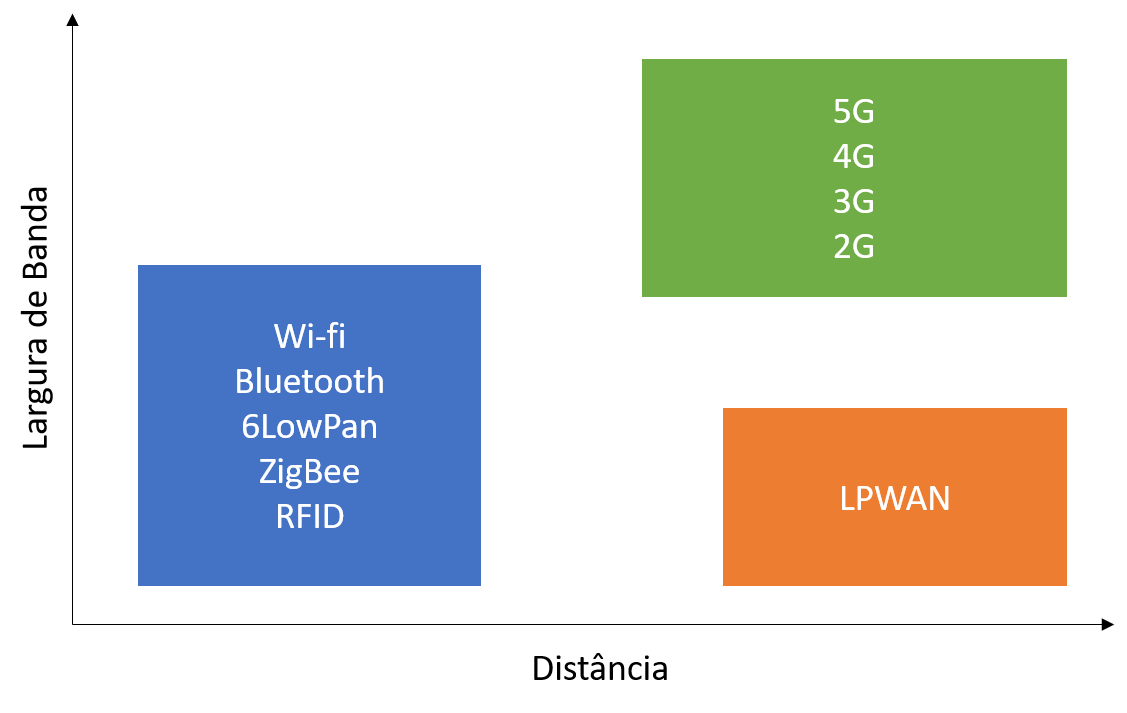
\includegraphics[width=0.45\textwidth]{images/lpwan.png}
\caption{Gráfico com relação Distancia vs Largura de Banda\cite{masterthesisLPWAN}}\label{figgraphlpwan}
\end{figure}



\section {Kea Tracker}\label{kea}
O Projeto Kea Tracker utiliza Beacon’s da Ruuvi, uma Beacon open-source\cite{ruuvi}, que disponibiliza de forma open-source tanto o Firmware para alterações, como as aplicações para Android e IOS. Será desenvolvida uma aplicação baseada na aplicação fornecida e o Firmware para disponibilizar a funcionalidade de data-logger.
\subsection{Beacons BLE}
\par
O Bluetooth Low Energy ou simplesmente BLE foi desenvolvido a pensar nos novos equipamentos IOT, onde os utilizadores querem vários equipamentos ligado ao mesmo tempo. Para tal foi desenvolvido o BLE que permite mais ligações ao mesmo tempo comparando com o Bluetooth clássico.
Como é indicado no nome, o principal fator diferenciador nesta versão, utilizada muitas vezes em equipamentos IOT, é o baixo consumo de aproximadamente metade relativamente ao Bluetooth normal. Outras características melhoradas a visar os equipamentos de IOT no BLE são a baixa largura de banda e o baixo tempo de transmissão.

Com o desenvolver do BLE foram criados, novos tipos de equipamentos, nomeadamente as beacons, equipamentos quase sempre alimentados por pilhas, que comunicam através de BLE, tornando o equipamento portátil. As beacons são caracterizadas por transmitir pequenas quantidades de informação em Broadcasting.
Existem dois tipos de beacons as beacons não conectáveis e as conectáveis\cite{blepacket}. Como indicado no nome as beacons conectáveis permitem que um equipamento (como um smartphone) se conecte á beacons e esta fica preparada para receber dados. As não conectáveis apenas permitem o broadcasting dos dados, poupando energia pois apenas é necessário ter o módulo acordado para fazer o broadcast e o restante do tempo podem estar num estado sleep. Na figura \ref{blepacket} é apresentado o pacote que é transmitido em broadcast para os outros equipamentos ao alcance.

\begin{figure}[htb]
\centering
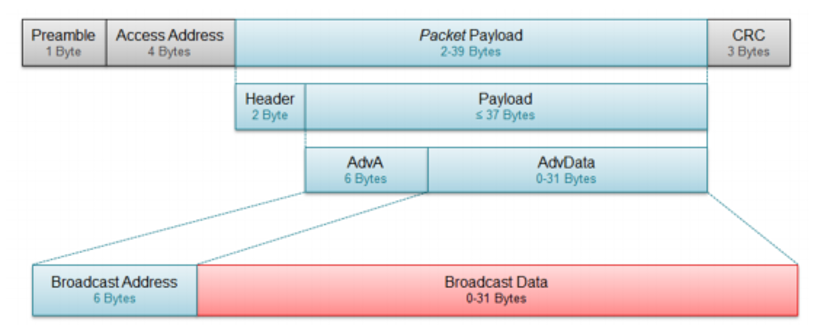
\includegraphics[width=0.65\textwidth]{images/blepacket.png}
\caption{BLE Broadcast packet\cite{blepacket}}\label{blepacket}
\end{figure}


\subsection{Ruuvi Beacons}
\par Neste projeto o firmware das beacons necessita de uma alteração, tornar a beacon numa beacon conectável e esta armazenar internamente as últimas leituras num buffer circular e criar um data-logger e caso o cliente pretenda poderá conectar mais tarde para fazer o download para aplicação e posterior envio para o Senslive, não necessitando a proximidade do smartphone á beacon durante todo o tempo. A Ruuvi dispõe de dois modos de desenvolvimento de firmware da beacon em C ou usando o Espruino, á semelhança do MicroPython um interpretador de JavaScript para microcontroladores lançado em 2012, totalmente compatível com as beacons da Ruuvi.
\subsection{Apps Smartphones}
Na fase inicial será adaptada a versão disponibilizada para Android para agilizar a integração com o portal Senslive. A aplicação base para android disponibilizada pela Ruuvi foi desenvolvida em Kotlin\cite{ruuviappgithub}, uma linguagem desenvolvida pela JetBrains multiplataforma e que inclui o Android nessas plataformas compatíveis.
De seguida estão apresentadas algumas alterações necessárias na aplicação:
\begin{itemize}
\item Alteração das Imagens e Logotipo da App;
\item Alteração do Nome da App;
\item Remoção de conteúdo não necessário;
\item Bloqueio do URL de envio para usar exclusivamente o portal Senslive;
\item Melhoramento da precisão da posição GPS;
\item Possibilidade da alteração dos intervalos de registo
\end{itemize}

\section {dot.Tracker}\label{dot}
Á semelhança do projeto Kea Tracker o projeto dot.Tracker usa igualmente beacon's BLE para enviar a informação necessária para o respetivo portal. É necessário recolher os pacotes recebidos das beacons enviá-los para o servidor e calcular a distância entre a beacon e o receptor e com o auxilio de múltiplos recetores realizar a triangulação da beacon num mapa. No decorrer do projeto será necessário desenvolver uma plataforma web para receber e visualizar as localizações provenientes das beacons e respetivas configurações, adotar o método de algoritmo para a triangulação da beacon relativamente a vários recetores e realizar testes ao funcionamento e precisão do sistema.
\subsection{Beacons e gateway}
 Para este projeto irá ser utilizado durante o desenvolvimento a solução da Beacon Line\cite{taskit} e posteriormente desenvolvido recetores propriétarios da Captemp. A solução apresentada pela Beacon Line, é composta por um gateway e vários nós. Cada nó possui um recetor BLE e quando o mesmo recebe um broadcast proveniente da beacon o transmite para o gateway. Caso exista alguma divergência da potência de transmissao desde o último pacote enviado por essa mesma beacon o gateway com connectividade Ethernet realiza o publish num broker onde é possível o servidor obter os pacotes das beacon's.



\section{Soluções e Tecnologias Disponíveis} \label{solucoesDisponiveis}
\subsection{Tecnologias Disponíveis}
\subsubsection{Compressão de Ficheiros}
\par
Atualmente a vida online do Homem passou a ter um grande impacto na sua vida. Para tal as páginas web e seus conteúdos foram aumentado em quantidade e tamanho e com menores tempos de resposta. Isso é aplicável tanto aos ficheiros que contem o layout da página, quer das imagens. Para poupar dados de transmissão e reduzir tempos de envios, ou simplesmente suportar larguras de banda inferiores, os browsers integraram a possibilidade de receber os ficheiros comprimidos e fazer a descompressão para mostrar ao cliente quase em tempo real. Atualmente os browser recentes suportam a compressão por GZIP( já utilizado na página do equipamento Nidus) e compressão utilizado a codificação Brotlin \cite{Alakuijala2019} \cite{brotlirfc}.
Cada método de compressão possui as suas vantagens e desvantagens, o brotli por sua vez á semelhança de outros métodos em comparação com o GZIP, tem uma taxa de compressão superior\cite{Alakuijala2015}, isto significa que consegue reduzir o mesmo ficheiro no seu respetivo ficheiro comprimido ocupando menos espaço em relação ao GZIP, mas como desvantagem o tempo de compressão do mesmo é superior. Ao contrário da compressão, na descompressão o Brotli tem melhores resultados do que nas restantes alternativas apresentando velocidades superiores de descompressão.
\par
O GZIP e o brotli usam na sua compressão para reduzir o tamanho do ficheiro o algoritmo de compressão LZ77, que procura sequências repetidas utilizando o método de janela deslizante e substitui essas sequências por referências para a primeira ocorrência que não foi substituída indicando a distância a que a primeira ocurência ocorre e o tamanho a substitui.
\par O sistema de janela deslizante define um tamanho da janela e ao deslocar a janela do tamanho definido define um dicionário. Após definir o dicionário com vários tamanhos de janelas, percorrer novamente o ficheiro através do método de janela deslizante novamente a procurar repetições das entradas que existem no dicionário. Quando uma sequência é encontrada esta é substituída  por uma referência da posição da primeira ocurrência da mesma. Na figura \ref{janela} é apresentado um exemplo do funcionamento da janela deslizante para a obtenção do dicionário com o tamanho da janela a variar de 2 a 7.
\begin{figure}[htb]
\centering
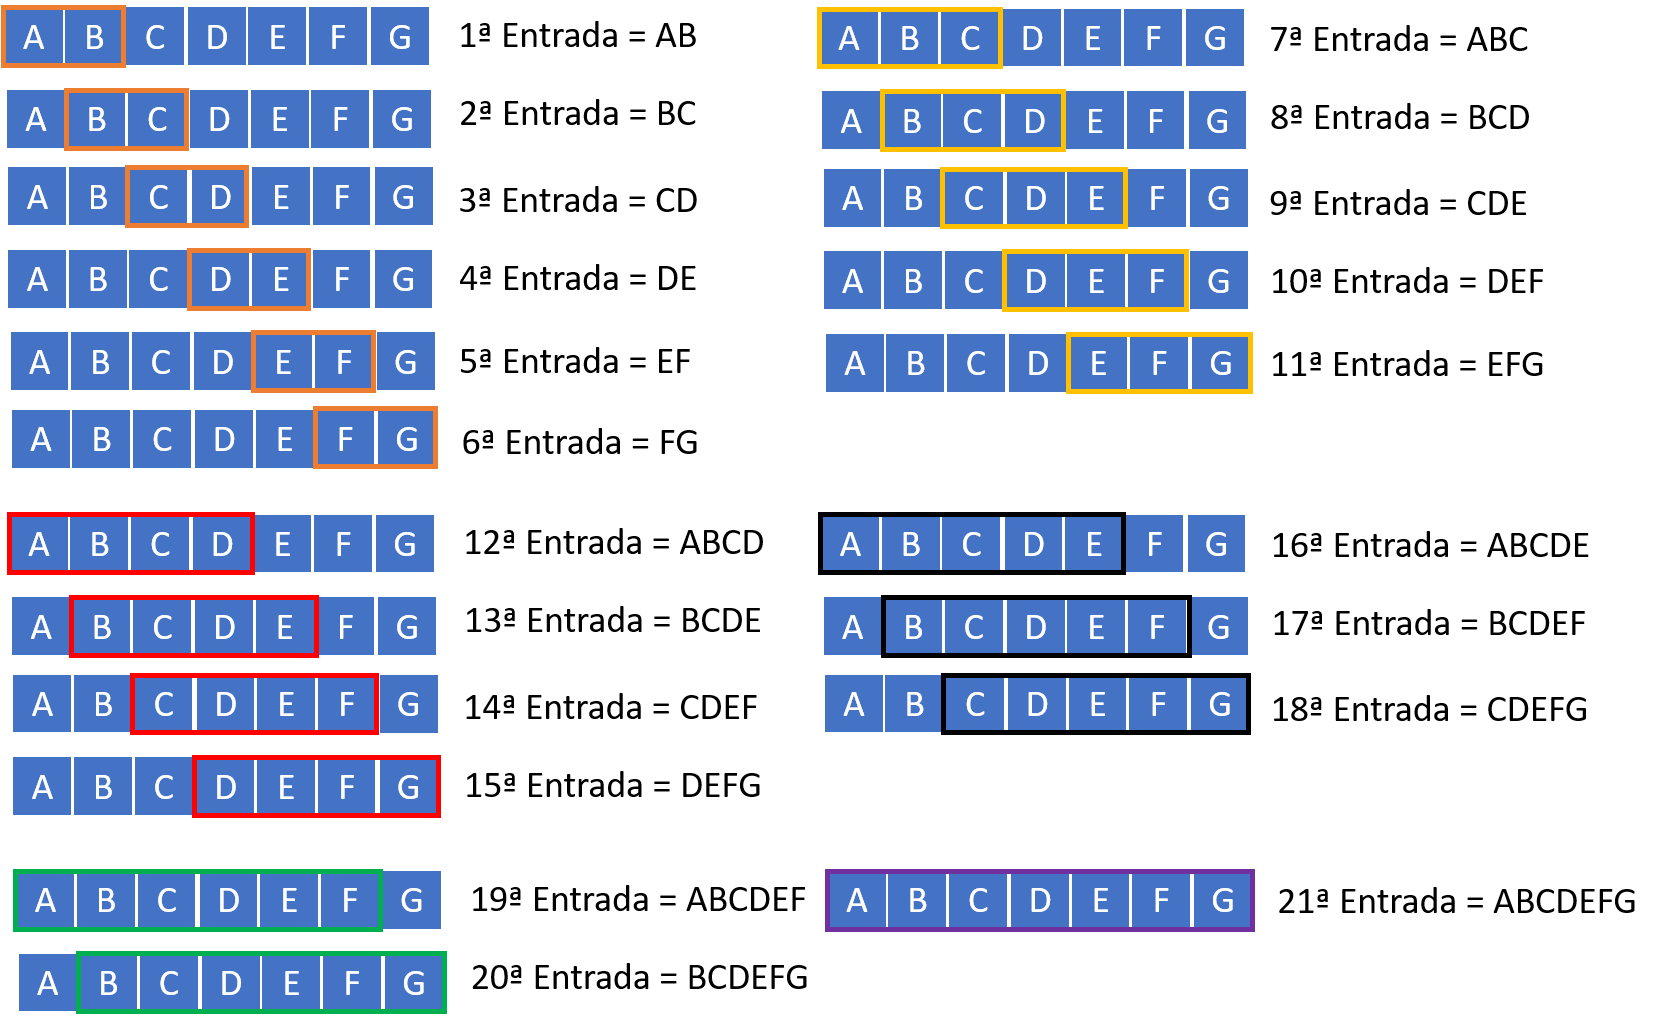
\includegraphics[width=0.85\textwidth]{images/janeladeslizantedicionario.png}
\caption{Funcionamento da Janela Deslizante}\label{janela}
\end{figure}


\par Na figura \ref{gzip} e \ref{gzip2} é apresentado dois exemplos visuais e simples utilizando frases de como o LZ277, usado pelo GZIP e Brotl através do sistema de janela deslizante procura as repetições e comprime os ficheiros. Na Figura \ref{unzip} é apresentado o ficheiro base, representado por um pequeno texto. No exemplo apresentado pela figura \ref{gzip} apenas foi utilizado a substituição de palavras inteiras, na figura \ref{gzip2} procura sequências de caracteres sejam elas palavras ou não. Nos exemplos apresentados a redução foi de 20\% [$1-\dfrac{48}{60}\times100\%$] no primeiro exemplo e de aproximadamente de 32\% [$1-\dfrac{41}{60}\times100\%$] no segundo.
\begin{figure}[htb]
\centering
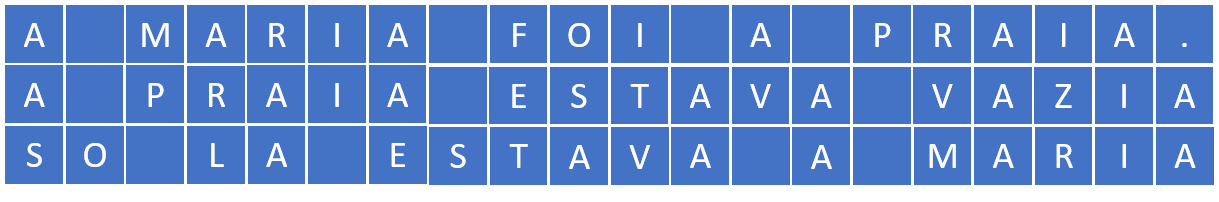
\includegraphics[width=0.85\textwidth]{images/FILE.png}
\caption{Sequência não comprimida}\label{unzip}
\end{figure}

\begin{figure}[htb]
\centering
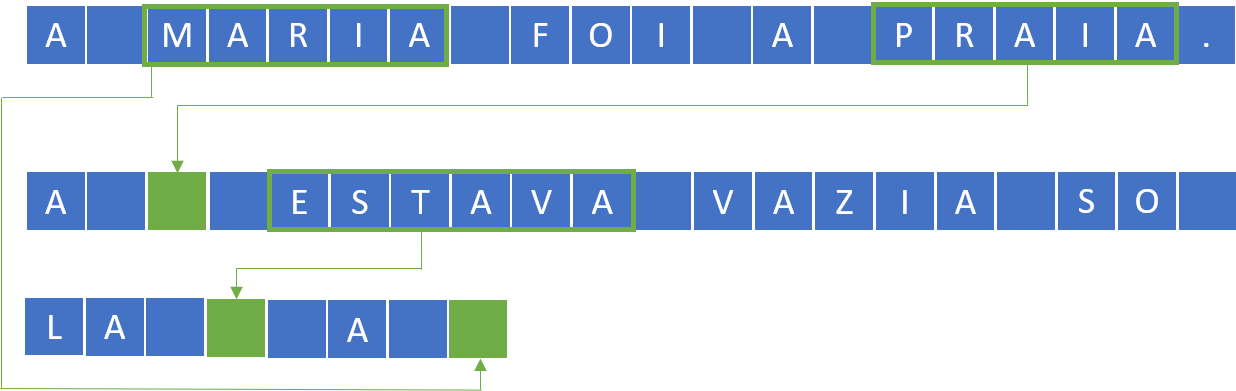
\includegraphics[width=0.85\textwidth]{images/gzip.png}
\caption{Sequência comprimida com LZ77 (apenas palavras)}\label{gzip}
\end{figure}
\begin{figure}[htb]
\centering
\includegraphics[width=0.85\textwidth]{images/gzip2.png}
\caption{Sequência comprimida com LZ77(palavras e sequências)}\label{gzip2}
\end{figure}


\subsubsection{Compressão de Imagens}
\par

O utilizador pretende igualmente ver as imagens com a máxima qualidade, mais qualidade significa um maior detalhe e por sequencia um ficheiro de maior tamanho. Existem atualmente vários softwares online e locais que reduzem o tamanho das imagens. Na conceção da página da Nidus é utilizado o website TinyPNG.com que analisa a imagem original e converte as cores em cores mais simples de o sistema armazenar, como por exemplo uma imagem com 24 bits de profundidade de cor pode ser convertido em uma similar com apenas 8 bits reduzindo o tamanho do ficheiro e impercetível para o olho humano num ecrã\cite{Hilles2019}. Alternativamente ao Tiny Png existem softwares, similares alguns de licença GNU/GPL, para comprimir imagens. Com o "Mass Image Compressor"\cite{Mass_Image_Compressor}(apenas um exemplo), é possível comprimir as imagens com a possibilidade de indicar a quantidade de compressão.
\par
Com a enorme quantidade e diversidade de monitores existentes, as páginas web necessitam de ser responsivas e apresentar a melhor imagem para o monitor em questão, isso normalmente traduz-se em várias versões similares da imagem alojadas no servidor. No caso dos microcontroladores e sistemas embebidos o espaço encontra-se limitado e deve-se arranjar uma solução. Uma solução possível é ao invés da utilização de imagens PNG, JPG ou outras, é a utilização de imagens em SVG, onde a imagem é representada por um ficheiro XML que descreve uma imagem bidimensional e utiliza na sua constituição modelos matemáticos para o cálculo das posições dos elementos. Com isto é possível manipular o XML em tempo real para alterar elementos ou remover, alterar cores, criar animações entre outras. Inclui a vantagem de como a imagem é representada por formulas matemáticas, é possível escalar a imagem sem perder qualidade, pois a função matemática é ajustável. Num sistema embebido como o caso da Nidus é vantajoso a utilização de imagens em SVG para criação das animações. Atualmente as animações da página da Nidus são criadas com várias imagens PNG comprimidas e convertidas em base64 e são alternadas no HTML pelo JavaScript. Com a utilização de imagens SVG é possível ter apenas uma imagem alojada e manipular a imagem em tempo real através do JavaScript de uma forma mais suave para o utilizador, pois apenas a zona a alterar é alterada na imagem.
Á semelhança dos JPG e PNG o SVG também pode ser comprimido, para tal basta no XML da imagem remover os meta-dados  e utilização de funções matemáticas mais simples, não necessários para o browser apresentar a representação gráfica do mesmo, mas os softwares de edição adicionam para funcionalidades exclusivas do editor. Á semelhança dos ficheiros HTML após a remoção dos meta-dados o ficheiro pode ser minificado.

\subsubsection{Localização indoor}
\par
É possivel encontrar na comunidade científica vários estudos sobre a utilização de redes Wi-Fi e Bluetooth para sistemas de localização. Estes mesmos focam-se no cálculo das distâncias do equipamento para vários recetores no mesmo intervalo temporal, algumas destas soluções baseiam-se nos valores de RSSI da transmissão e o valor definido como constante da potência de transmissão á distância de 1 metro, e estimar a sua distância aproximada de cada recetor, com essas aproximações é possivel através do algoritmo escolhido\cite{Wang2013}, obter a estimativa da localização do equipamento e a sua colocação num mapa.
A distância de um recetor para o emissor baseada no  valor de RSSI é expressa pela seguinte formula, onde dbm é a constante da potência de transmissão da beacon a 1 metro, n a constante do ambiente e o RSSI corresponde ao RSSI da transmissão:
\par
\begin{center}
  $d=10^(\frac{dbm-RSSI}{10 \times n})$
\end{center}

\par
Após a obtenção da distância para cada recetor é possível  aplicar um algoritmo para estimar a localização. Os mais referenciados e adotados são o centroid baseado no centro geométrico do polígono formado pelas interceções das circunferências criadas com o raio da distância calculada pela fórmula anteriormente apresentada, o método Three-border Positioning e o Least Square Estimation.
Como é possivel observar na figura \ref{centroid} utilizando o método do centroid, o centro geométrico corresponde á localização do equipamento com base nos recetores. A formula que representa o centro utilizando o centroid é expressa pela seguinte equação onde n representa o numero de recetores utilizados no cálculo.
\par
\begin{center}
$ (x,y)= (\frac{x_{1}+x_{2}+x_{3}+...+x_{n}}{n},\frac{y_{1}+y_{2}+y_{3}+...+y_{n}}{n})$
\end{center}

\begin{figure}[htb]
\centering
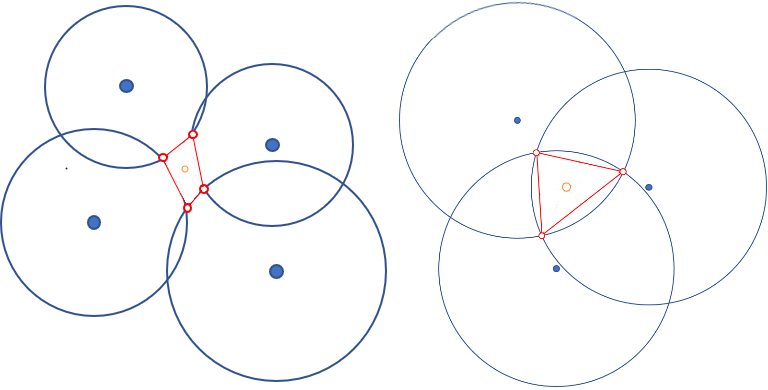
\includegraphics[width=0.95\textwidth]{images/centroid3.png}
\caption{Posição utilizando o método Centroid com 3 e 4 recetores}\label{centroid}
\end{figure}

Ao invés da utilização do método do centroid se for adotado o método Three-border Positioing, é criada a função definida por ramos composta pelas três equações da circunferência A, B e C com os respetivos centros em cada recetor e com o raio igual á distância calculada para esse mesmo recetor. Para calcular a posição estimada é calculado o resultado dessa mesma função de modo a encontrar o ponto x,y que representa a posição do equipamento.
\par 
Utilizando o método Least Sqare Estimation ou simplesmente LSE e á semelhança do Three-border Position\cite{Zhu2014} é criada a função de ramos das equações das circunferências dos vários recetores com o raio da distância calculada, mas pode igualmente como o centroid utilizar mais do que três recetores aumentando a precisão. \par Hua, Z., Hang, L., Yue, L., Hang, L., \& Kan, Z. (2014). Geometrical constrained least squares estimation in wireless location systems. 2014 4th IEEE International Conference on Network Infrastructure and Digital Content. apresenta os passos necessários calcular a posição X do equipamento através do método LSE. Em primeiro são criadas a função de ramos composta pelas equações das circunferências com centro nos recetores ([$x_{1}$,$y_{1}$],[$x_{2}$,$y_{2}$],[$x_{3}$,$y_{3}$],[$x_{4}$,$y_{4}$]) e o raio igual á distância calculada($d_{1}$,$d_{2}$,$d_{3}$,$d_{4}$).
\begin{center}
\[
  \begin{cases}
      (x_{1} -x)^2 + (y_{1}-y)^2 = {d_{1}}^2\\
      (x_{2} -x)^2 + (y_{2}-y)^2 = {d_{2}}^2\\
      (x_{3} -x)^2 + (y_{3}-y)^2 = {d_{3}}^2\\
      (x_{4} -x)^2 + (y_{4}-y)^2 = {d_{4}}^2\\
  \end{cases}
\]
\end{center}

\par Após a criação da função é subtraido o primeiro ramo aos restantes ramos e a função reduz o numero de ramos para n-1 onde n representa o numero de recetores a usar na função.
\begin{center}

\[
  \begin{cases}
     2(x_{2}-x_{1})x+2(y_{2}-y_{1})y={x_{2}}^2-{x_{1}}^2+{y_{2}}^2-{y_{1}}^2+{d_{2}}^2+{ d_{1}}^2\\
     2(x_{3}-x_{1})x+2(y_{3}-y_{1})y={x_{3}}^2-{x_{1}}^2+{y_{3}}^2-{y_{1}}^2+{d_{3}}^2+{ d_{1}}^2\\
     2(x_{4}-x_{1})x+2(y_{4}-y_{1})y={x_{4}}^2-{x_{1}}^2+{y_{4}}^2-{y_{1}}^2+{d_{4}}^2+{ d_{1}}^2\\
  \end{cases}
\]
\end{center}
\par A função pode ser representada pelo seu equivalente numa representação de matrizes por $2AX = b$ onde.

\begin{center}



$A=\begin{bmatrix}
x_{2}-x_{1} & y_{2}-y_{1}\\
x_{3}-x_{1} & y_{3}-y_{1}\\
x_{4}-x_{1} & y_{4}-y_{1}
\end{bmatrix}$

$B=\begin{bmatrix}
b_{1}\\
b_{2}\\
b_{3}
\end{bmatrix}=\begin{bmatrix}
{x_{2}}^2-{x_{1}}^2  + {y_{2}}^2-{y_{1}}^2 - {d_{2}}^2 + {d_{1}}^2 \\
{x_{3}}^2-{x_{1}}^2  + {y_{3}}^2-{y_{1}}^2 - {d_{3}}^2 + {d_{1}}^2 \\
{x_{4}}^2-{x_{1}}^2  + {y_{4}}^2-{y_{1}}^2 - {d_{4}}^2 + {d_{1}}^2 \\
\end{bmatrix} $

\end{center}

\par A posição estimada do equipamento representada no exemplo por X é definida por:



\par
\begin{center}
$ X= \frac{1}{2}(A^T A)^{-1} A^T b$
\end{center}

\par Os testes analisados demonstram\cite{Wang2013} , que o método LSE é o método que obtem os melhores resultados com os valores mais próximos do real. No teste apresentado em segundo lugar está o Three-border Position e por último o Centroid. Com algumas discrepâncias em algumas das amostragens.

\subsection{Produtos Similares}
\subsubsection{NB-Iot}
\par
Atualmente no mercado começam a surgir alguns produtos similares ao que se pretende desenvolver como é o caso dos sensores da Efento\cite{epoka}, que disponibiliza vários tipos de sensores que comunicam por NB-Iot. A Efento é uma empresa fundada em 2014 e é focada em desenvolvimento de equipamentos IOT. Atualmente desenvolveram versões com suporte para NB-Iot. Estes equipamentos tem a desvantagem de não ser compatível com o pacote de envio desenvolvido no portal Senslive e apenas permite o envio para o portal da Efento e não existe a possibilidade da utilização das sondas já comercializadas pela Captemp. Como vantagem á semelhança do equipamento a desenvolver é a utilização de um sistema com Log para quando não existe possibilidade de comunicação.
Devido ao desenvolvimento da tecnologia ainda existem poucas soluções em comercialização, estando as mesmas em desenvolvimento. A Captemp possui igualmente outro equipamento, completamente desenvolvido pela empresa, em desenvolvimento que tira partido do NB-Iot com o acréscimo em relação ao que se pretende desenvolver durante o estágio, a possibilidade de ter mais sensores, maior capacidade de Log interno, configuração por Bluetooth, GPS e um Display integrado como extra.
\subsubsection{Kea Tracker}
Após pesquisas online é possível encontrar algumas soluções de beacons que permitem o armazenamento interno de leituras para desenvolver um sistema de data-logger tais como a Beacon da Fujitsu, a FWM8BLZ02A-109069\cite{beacon1} , á semelhança da beacon da Ruuvi usa o mesmo chip o nRF52832 da Nordic Semiconductor, mas apresenta como vantagens a inclusão de um sistema de Logs interno com capacidade para aproximadamente 4080 leituras e a diversidade de sensores já incluídos. Como desvantagem em relação á Beacon da Ruuvi tem a inclusão de um sensor de temperatura ao invés de temperatura e humidade, não possui sensor de pressão atmosférica e não é open-source possuindo um firmware fechado. A vantagem de se desenvolver um produto desde a sua raiz é a possibilidade de ter o controlo total sobre a solução para posteriores melhoramentos e ter a solução a desempenhar apenas o que pretendemos.
\par
Outra solução existente no mercado é igualmente a solução da Blue Maestro que possui variadas versões de beacons. Á semelhança da Beacon da Fujitsu possuem igualmente sistema de Log. Contrariamente á FWM8BLZ02A-109069 é uma beacon que tem disponível em Open-Source uma API e um SDK para desenvolver as nossas aplicações. Comparada com a beacon da Ruuvi, a Ruuvi beacon é completamente open-source e não apenas a API para comunicação.
\par
Na tabela \ref{tabbeacons} são apresentadas as diferenças e semelhanças entre os três modelos analisados

\begin{table}[htb]
\caption{Comparação entre beacons \cite{specsrect}\cite{bluespecs}\cite{ruuvispecs}}\label{tabbeacons}
\begin{tabular}{|c|c|c|c|}\hline
& Ruuvi Tag& Fujitsu Beacon &Blue Maestro \\\hline
Processador& nRF52832& nRF52832 &? \\\hline
Memória&\begin{tabular}{@{}c@{}}512kB Flash \\ 64kB RAM\end{tabular} & 32K Não volátil &?\\\hline 
Protocolos&\begin{tabular}{@{}c@{}c@{}@{}c@{}} Bluetooth 5 \\ Wirepass \\ Mira OS\\QUUPA\\Others (2.4GHz)\end{tabular}&Bluetooth 4.1&BLE 4.2\\\hline 
\begin{tabular}{@{}c@{}}Potência de\\ Transmissão\end{tabular} &+4 dBm &\begin{tabular}{@{}c@{}}-16, -12, -8\\ -4, 0, +4 dBm\end{tabular} &-4, 0, +4 dBm \\\hline
Sensores& \begin{tabular}{@{}c@{}c@{}c@{}} Acelerometro\\ Temperatura\\ Humidade \\Pressão\end{tabular} &\begin{tabular}{c@{}c@{}} Acelerómetro\\ Temperatura\end{tabular}&\begin{tabular}{@{}c@{}c@{}} Temperatura\\ Humidade \\Pressão\end{tabular}\\\hline 
NFC & \checkmark&- &-\\\hline
Bateria &\begin{tabular}{@{}c@{}}CR2477\\ 1000mAH - Li/MnO2\end{tabular}&CR2450 &CR2032\\\hline
\begin{tabular}{@{}c@{}}Autonomia\\(espetável)\end{tabular}& ~10 Anos&1 Ano em Broadcast &\begin{tabular}{@{}c@{}}1 Ano em Broadcast\\2 Anos com Log\end{tabular}\\\hline
Data Logger &\begin{tabular}{@{}c@{}}-\\(a desenvolver)\end{tabular}&\checkmark &\checkmark\\\hline
Open Source & \checkmark&- &\checkmark ( API \& SDK )\\\hline
Informações & \begin{tabular}{@{}c@{}c@{}@{}} IP67 \\ 2 Botões\\2 Leds\\52mm \diameter\\\end{tabular}&\begin{tabular}{c@{}c@{}} Led\\ 40 x 31 x 12mm \end{tabular}&\begin{tabular}{@{}c@{}}24000 Registos\\33mm \diameter\end{tabular} \\\hline
\end{tabular} 
\end{table}
\par




\chapter{Conclusões}
\par Inserido num contexto empresarial , e tratando-se de projetos em desenvolvimento e de desenvolvimento contínuo, estes não foram concluidos com o concluir deste relatório e estágio. Todos os objetivos defindos no inicio do estágio foram concluidos com sucesso e com bons resultados como apresentado no capítulo \ref{cap4}. 
\par A realização de um estágio com projetos reais em ambiente empresarial permitiu uma melhor compreensão dos vários fatores que  não são possiveis replicar em ambiente académico, além da utilizaão de novas metodologias e técnologias.

\par Para trabalho futuro prevê-se a implementação do plugin Blockly na página da Nidus, algumas alterações simples de Design na página e a reformulação da ferramenta de compressão da página para a utilização do Brotli.
O projeto do Nb-Iot caso exista atualizações de \textit{Firmware} por parte da Digi que permitam a comunicação por Bluetooth, será implementada a configuração do equipamento através de uma aplicação móvel. No projeto dot.Tracker caso a necessidade de aumentar a precisão se venha a verificar, deve-se ponderar a migração para um sistema diferente de localização indoor sem recurso ao valor de RSSI tal como o \textit{Bluetooth} 5.1, em desenvolvimento, especialmente desenhado para localização em ambientes fechados. O \textit{Bluetooth} 5.1 com recurso a várias antenas por recetor, consegue calcular o ângulo entre o emissor e o recetor e com recurso a vários recetores delimitar a posição do emissor.

\par A utilização de \textit{Frameworks} que permitam o desenvolvimento de aplicações multiplataforma, tais como a utilizada neste estágio, o IONIC, é uma mais valia, pois utilizando o mesmo código fonte desenvolvido, permite além de manter o Design similar entre as plataformas, diminui o tempo de desenvolvimento quando são necessárias correções e atualizações e caso não seja necessário pelos requiesitos da aplicação, abstrai o desenvolvimento da programação nativa em cada ambiente, para \textit{Frameworks} de mais alto nível.

\par O estágio na Captemp foi uma experiência enriquecedora, onde foi possivel obter e consolidar conhecimento já adquiridos e novos, experiência e criadas novas relações quer a nível profissional quer pessoal.

% REFERENCES
% Edit the references.bib file to add your own references, that you can then
% \cite on your text.


\bibliographystyle{ieeetr}

\addcontentsline{toc}{chapter}{Bibliografia}
\bibliography{references}

%\clearpage %\cleardoublepage %for openright
\renewcommand{\thesection}{Apêndices \Roman{section}}

\begin{appendices}

\end{appendices}

\end{document}
